%\documentclass[aspectratio=54]{beamer}
\documentclass[handout,aspectratio=54]{beamer}
\usepackage{amsmath, amssymb}
%\usepackage[utf8]{inputenc}
%\usepackage{zxjatype}
%\usepackage[ipa]{zxjafont}

\usepackage{mymacro}

\usefonttheme{professionalfonts}
\setbeamertemplate{navigation symbols}{}

% --- page number ---
\setbeamertemplate{footline}{%
	\raisebox{10pt}{\makebox[\paperwidth]{\hfill\makebox[7em]{\normalsize\texttt{\insertframenumber/\inserttotalframenumber}}}}%
}

\mode<presentation>
{
\usetheme{Madrid}
}

%%%%%%%%%%%%%%%%%%%%%%%%%%%%%%%%%%%%%%%%%%%%%%%%%%%
\title[]{Zero-Order,Black-Box,Derivative-Free,and\\
Simulation-Based Optimization
}%Subspace Methods: Balance between Optimization problem and the Subproblem}

\author[Stefan Wild]{Stefan Wild}

\institute[ANL]{
Argonne National Laboratory\\
Mathematics and Computer Science Division
}

\date[August 5, 2016]{August 5, 2016}


\usepackage{graphicx}
\usepackage{subfigure}
%\batchmode
\usepackage{amsmath,amssymb,enumerate,epsfig,bbm,calc,color,ifthen,capt-of,comment}



\usepackage{tcolorbox}
\usepackage{multicol}
\usepackage{color,xcolor,tikz}
\usepackage{graphicx}
%\usepackage{algorithm,algorithmic}
\usepackage{algorithmic}
\usepackage{algorithm}
\usepackage{amsthm}
\usepackage{subfigure}
\usepackage{graphicx}
\usepackage{comment}
\usepackage{tikz}
\usetikzlibrary{positioning}
\usetikzlibrary{chains}
\usepackage{pgf,tikz,pgfplots}
\pgfplotsset{compat=1.15}
\usepackage{mathrsfs}
\newtheorem{proposition}{Proposition}
\usetikzlibrary{arrows}
\usetikzlibrary{trees}
\usepackage{subfigure}

%\usepackage{xeCJK}
%\setCJKmainfont{SimSun}
\usepackage{hyperref}
\hypersetup{hidelinks}

\setbeamertemplate{theorems}[numbered]
%\numberwithin{subsection}{section}
%\numberwithin{theorem}{subsection}
\numberwithin{theorem}{section}


\usepackage[
backend=bibtex,
style=alphabetic,
citestyle=authoryear
]{biblatex}

\addbibresource{slides.bib} %Imports bibliography file
\AtBeginBibliography{\tiny}

\setbeamerfont{footnote}{size=\tiny}


%\usepackage{tikz}

\usetikzlibrary{mindmap}
\usepackage{verbatim}

\tikzset{level 1 concept/.append style={level distance = 25mm}}
\tikzset{level 2 concept/.append style={level distance = 15mm}}
\tikzset{level 3 concept/.append style={level distance = 15mm}}
\tikzset{every node/.append style={scale=0.6}}
\usetikzlibrary{positioning}
\usetikzlibrary{chains}
\usepackage{pgf,tikz,pgfplots}
\pgfplotsset{compat = newest}
\usepackage{mathrsfs}
\usetikzlibrary{arrows}
\usetikzlibrary{trees}
\usepackage{subfigure}


\definecolor{blue}{RGB}{38,28,163}

\usepackage{anyfontsize}

\usepackage{setspace}

\newtheorem{assumption}{Assumption}[section]

\usepackage{xcolor}

\AtBeginSection[]
{
\begin{frame}{The Plan}
\tableofcontents[currentsection]
\end{frame}
}

%%%%%%%%%%%%%%%%%%%%%%%%%%%%%%%%%%%%%%%%%%%%%%%%%%%%%%%%%%%%%

\begin{document}
\frame{\titlepage}

\begin{frame}{The Plan}
\tableofcontents
\end{frame}


\section{Motivation}

%2
\begin{frame}{Simulation-Based Optimization}
\begin{equation*}
\underset{x\in \mathbb{R}^n}{\mathrm{min}}\{f(x)=F[x,\textcolor{red}{S(x)}]:c_I[x,\textcolor{red}{S(x)}]\le0,c_E[x,\textcolor{red}{S(x)}]=0\}
\end{equation*}

\begin{itemize}
\item $S$ (numerical) simulation output, often \textcolor{red}{“noisy”} (even when deterministic)
\item Derivatives $\nabla_x S$ often \textcolor{red}{unavailable or prohibitively expensive to obtain/approximate directly}
\item $S$ can contribute to objective and/or constraints
\item Single evaluation of $S$ could take seconds/minutes/hours/days
\flushright{\textcolor{red}{Evaluation is a bottleneck for optimization}}
\end{itemize}

\colorbox[rgb]{0.5,0.6,0.7}{\textcolor{white}{Functions of complex numerical simulations arise everywhere}}

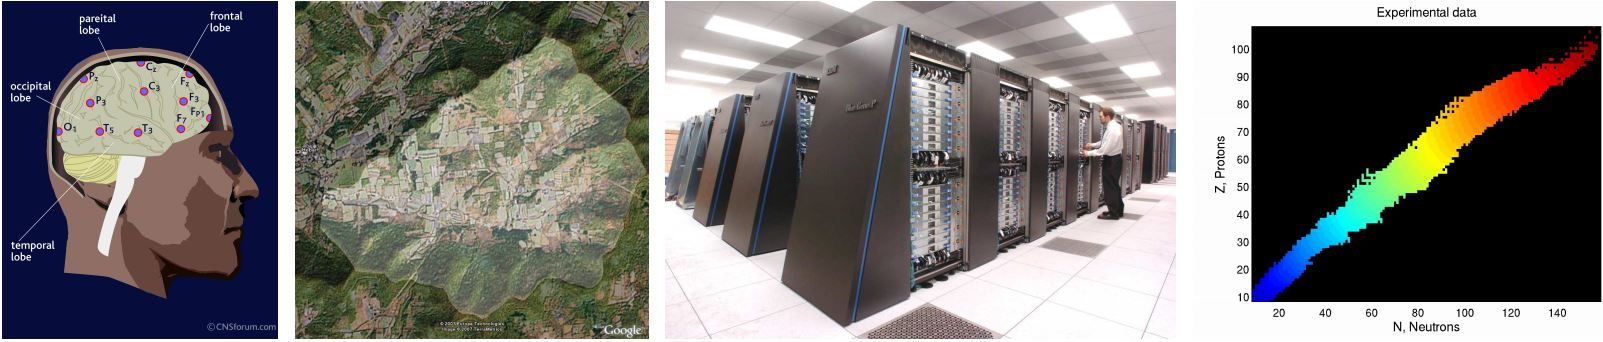
\includegraphics[width=\textwidth]{fig/2.jpg}
\end{frame}

%3
\begin{frame}{Computing is Responsible for Pervasiveness of Simulations in Sci\&Eng}
\begin{columns}
\column{0.3\textwidth}
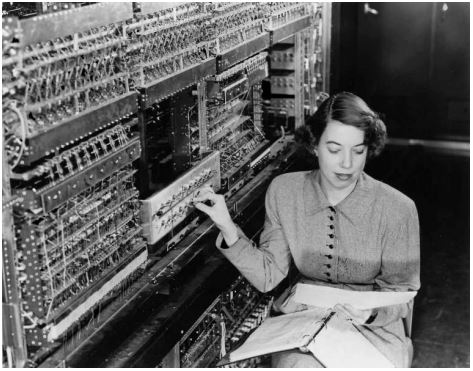
\includegraphics[width=\textwidth]{fig/3-1.jpg}
{
\scriptsize
Argonne’s AVIDAC\\
(1953: \textcolor{blue}{vacuum tubes})
}
\column{0.3\textwidth}
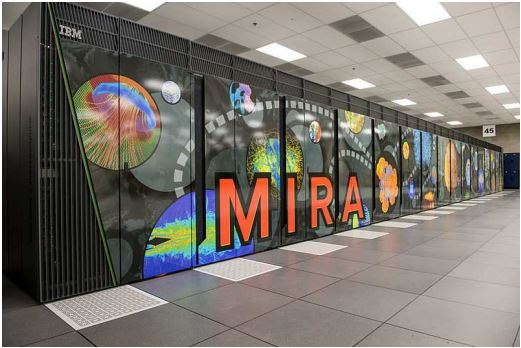
\includegraphics[width=\textwidth]{fig/3-2.jpg}
{
\scriptsize
Argonne’s Blue Gene/Q (2012: \textcolor{blue}{786,432 cores})\\
Currently \textcolor{blue}{6th} fastest in the world
}
\column{0.3\textwidth}
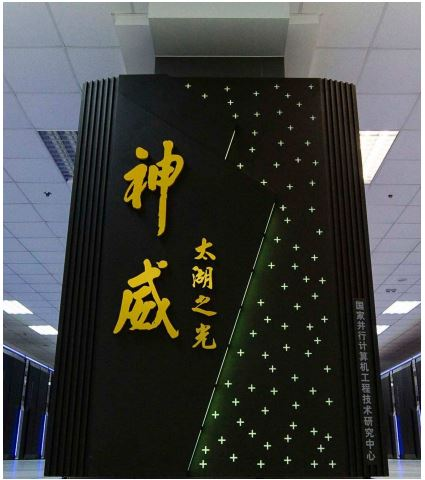
\includegraphics[width=\textwidth]{fig/3-3.jpg}
{
\scriptsize
Sunway TaihuLight (2016: \textcolor{blue}{11M cores})
Currently \textcolor{blue}{fastest} in the world
}
\end{columns}

\begin{itemize}
\item  Parallel/multi-core environments increasingly common
\begin{itemize}
\item Small clusters/multi-core desktops/multi-core laptops pervasive
\item Leadership class machines increasingly parallel
\end{itemize}

\item Simulations (the “forward problem”) become faster/more realistic/more complex
\end{itemize}
\end{frame}

%4-1
\begin{frame}{Improvements from Algorithms Can Trump Those From Hardware}
\begin{columns}
\column{0.7\textwidth}
Martin Gr$\ddot{\textup{o}}$tschel’s production planning benchmark problem (a MIP):\\
\textcolor{cyan}{1988} solve time using current computers and LP algorithms: \\
\textcolor{cyan}{2003} solve time using current computers and LP algorithms:

\column{0.2\textwidth}
{
\LARGE
82 years\\
1 minute
}
\end{columns}

\begin{itemize}
\item Speed up of \textcolor{blue}{43,000,000X}\\
$10^3$X from processor improvements\\
$10^4$X additional from \textcolor{blue}{algorithmic improvements}
\end{itemize}
\end{frame}

%4-2
\begin{frame}{Improvements from Algorithms Can Trump Those From Hardware}
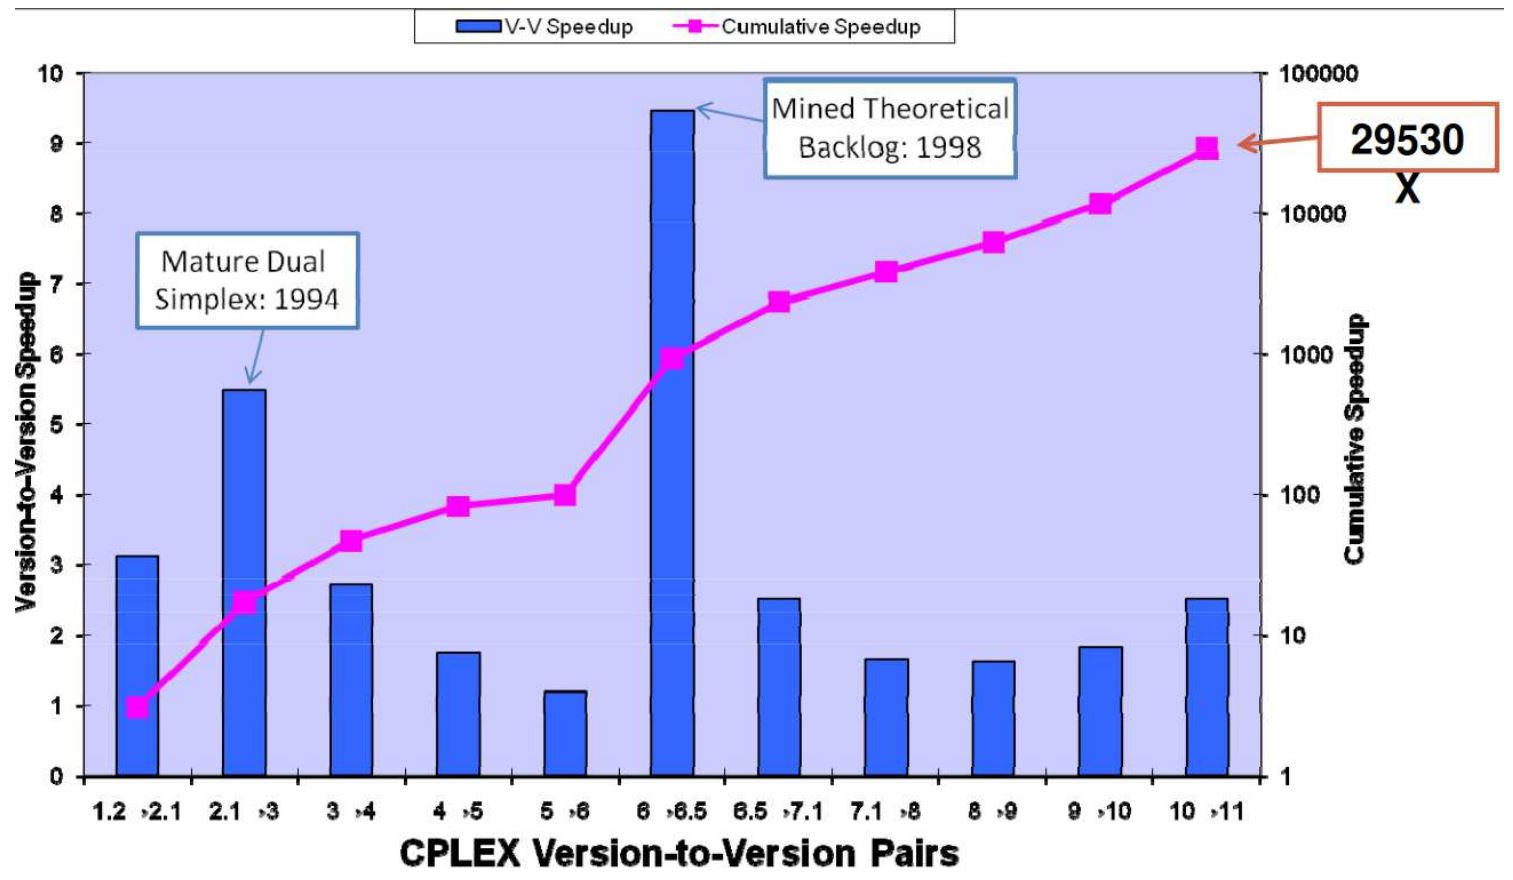
\includegraphics[width=\textwidth]{fig/4.jpg}
\centerline{
1991 (v1.2) to 2007 (v11.0): Moore’s Law transistor speedup: $\approx$ 256X
}
\centerline{
[\textcolor[RGB]{128,0,128}{Slide from Bixby (CPLEX/GUROBI)}]: Solves 1,852 MIPs
}
\end{frame}

%5-1
\begin{frame}{Derivative-Free/Zero-Order Optimization}
\centerline{
“Some derivatives are unavailable for optimization purposes”
}
\vspace{7.5cm} 
\end{frame}

%5-2
\begin{frame}{Derivative-Free/Zero-Order Optimization}
\centerline{
“Some derivatives are unavailable for optimization purposes”
}
\vspace{0.1cm} 
\colorbox[rgb]{0.5,0.6,0.7}{\textcolor{white}{The Challenge: Optimization is tightly coupled with derivatives}}\\
\vspace{0.1cm} 
Typical optimality \textcolor{blue}{(no noise, smooth functions)}
\begin{equation*}
\nabla_x f(x^*)+\lambda^T\nabla_x c_E(x^*)=0,c_E(x^*)=0
\end{equation*}

\begin{columns}
\column{0.35\textwidth}
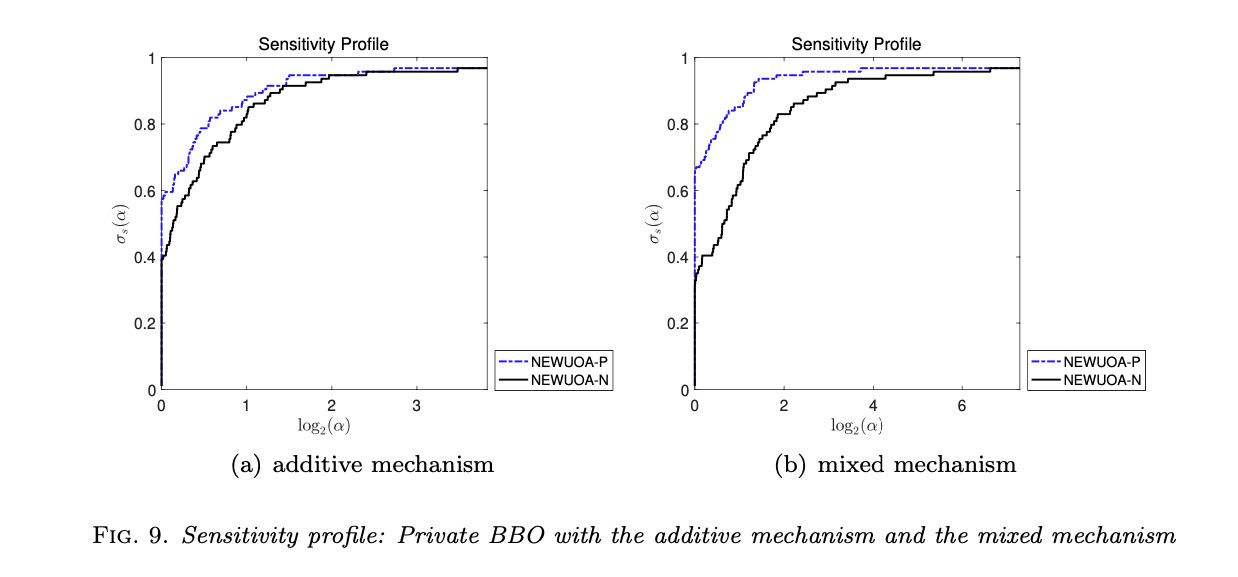
\includegraphics[width=\textwidth]{fig/5.jpg}

\column{0.6\textwidth}
(sub)gradients $\nabla_x f,\nabla_x c$ enable:

\begin{itemize}
\item Faster feasibility

\item Faster convergence
\begin{itemize}
\footnotesize{
\item Guaranteed descent
\item Approximation of nonlinearities
}
\end{itemize}

\item Better termination
\begin{itemize}
\footnotesize{
\item Measure of criticality

$||\nabla_x f||$ or $|| \mathcal{P}_\Omega(\nabla_x f)||$
}
\end{itemize}

\item Sensitivity analysis
\begin{itemize}
\footnotesize{
\item Correlations, standard errors, UQ, . . .
}
\end{itemize}
\end{itemize}
\end{columns}
\end{frame}

%6
\begin{frame}{Ways to Get Derivatives}
\begin{columns}
\column{0.6\textwidth}
\colorbox[rgb]{0.5,0.6,0.7}{\textcolor{white}{Handcoding (HC)}}\\
\vspace{0.1cm} 
“Army of students/programmers”
\begin{itemize}\footnotesize
\item[\textcolor{red}{?}] Prone to errors/conditioning
\item[\textcolor{red}{?}] Intractable as number of ops increases
\end{itemize}

\colorbox[rgb]{0.5,0.6,0.7}{\textcolor{white}{Algorithmic/Automatic Differentiation (AD)}}\\
\vspace{0.1cm} 
“Exact$^*$ derivatives!”
\begin{itemize}\footnotesize
\item[\textcolor{red}{?}]  No black boxes allowed
\item[\textcolor{red}{?}]  Not always automatic/cheap/well-conditioned
\end{itemize}

\colorbox[rgb]{0.5,0.6,0.7}{\textcolor{white}{Finite Differences (FD)}}\\
\vspace{0.1cm} 
“Nonintrusive”
\begin{itemize}\footnotesize
\item[\textcolor{red}{?}]  Expense grows with $n$
\item[\textcolor{red}{?}]  Sensitive to stepsize choice/noise
\end{itemize}

\column{0.4\textwidth}
\scriptsize{\textcolor{blue}{(assuming they exist)}}

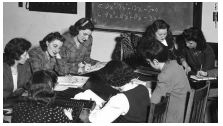
\includegraphics[width=\textwidth]{fig/6-1.jpg}

\includegraphics[width=0.4\textwidth]{fig/6-2.jpg}

\includegraphics[width=0.4\textwidth]{fig/6-3.jpg}
\end{columns}

\centerline{
\scriptsize{
\textcolor{blue}{$\rightarrow$}\textcolor[RGB]{128,0,128}{[Mor$\acute{\textup{e}}$ \& W.; SISC 2011], [Mor$\acute{\textup{e}}$ \& W.; TOMS 2012]}
}}
\centerline{
\footnotesize{
\textcolor{blue}{. . . then apply derivative-based method (that handles inexact derivatives)}
}}
\end{frame}

%7
\begin{frame}{Algorithmic Differentiation}
\flushright{
\scriptsize{
\textcolor{blue}{$\rightarrow$}
\textcolor[RGB]{128,0,128}{[$\underline{\textup{Coleman \& Xu}}$; SIAM 2016], [$\underline{\textup{Griewank \& Walther}}$; SIAM 2008]}
}
}

\begin{columns}
\column{0.6\textwidth}
\colorbox[rgb]{0.5,0.6,0.7}{\textcolor{white}{Computational Graph}}
\begin{itemize}
\item  $y=sin(a*b)*c$
\item  Forward and reverse modes
\item  AD tool provides code for your derivatives
\end{itemize}
\textcolor{blue}{Write codes and formulate problems with AD in mind!}

\column{0.3\textwidth}
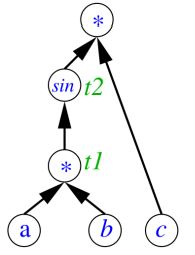
\includegraphics[width=\textwidth]{fig/7.jpg}
\end{columns}

\rule{\textwidth}{1pt}

\small\flushleft
Many tools (see \url{www.autodiff.org}):

\begin{table}[]\scriptsize
\begin{tabular}{rlrl}
\textcolor{cyan}{F}     & \textcolor{blue}{OpenAD} & \textcolor{cyan}{Matlab}   & \textcolor{blue}{ADiMat}, \textcolor{blue}{INTLAB}\\
\textcolor{cyan}{F/C}   & \textcolor{blue}{Tapenade}, \textcolor{blue}{Rapsodia} & \textcolor{cyan}{Python/R} & \textcolor{blue}{ADOL-C}        \\
\textcolor{cyan}{C/C++} & \textcolor{blue}{ADOL-C}, \textcolor{blue}{ADIC}      &&
\end{tabular}
\end{table}

\small\flushright
Also done in \textcolor{blue}{AMPL},\textcolor{blue}{GAMS},\textcolor{blue}{JULIA}!
\end{frame}

%8-1
\begin{frame}{The Price of Algorithm Choice: Solvers in PETSc/TAO}
\begin{columns}
\column{0.5\textwidth}
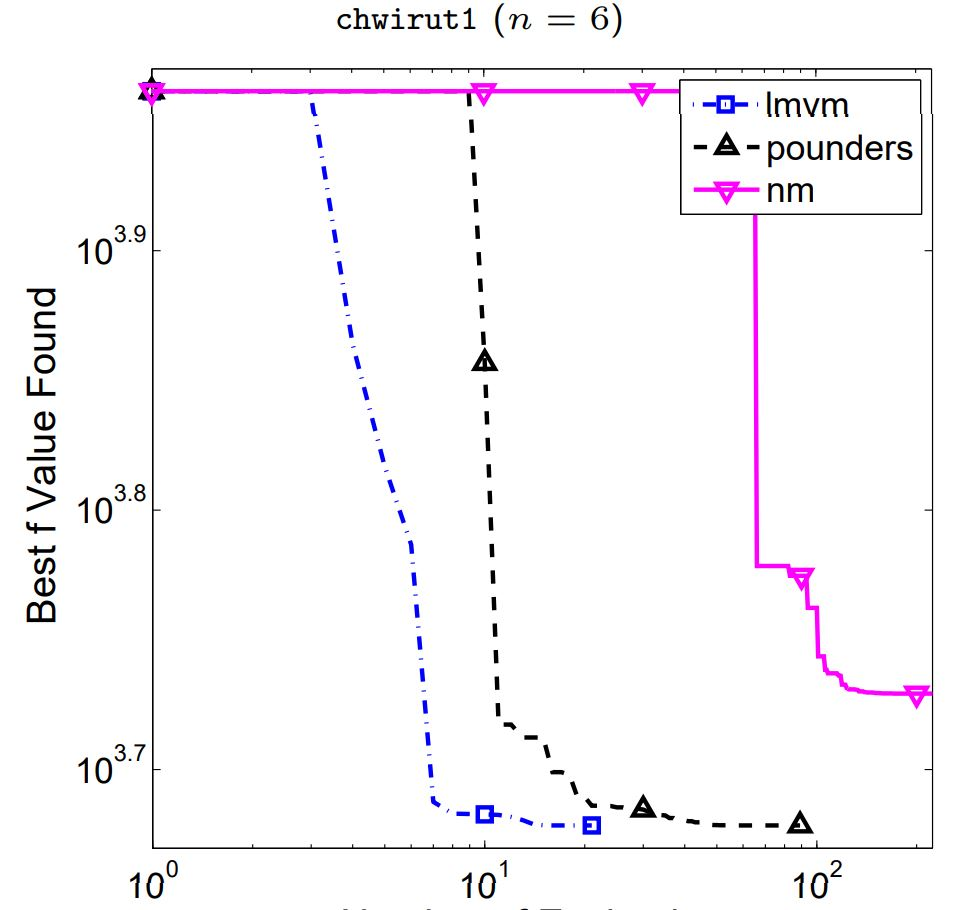
\includegraphics[width=\textwidth]{fig/8.jpg}
\begin{center}
Number of Evaluations
\end{center}

\column{0.5\textwidth}
\flushright{
\scriptsize{
Toolkit for Advanced Optimization\\
\textcolor[RGB]{128,0,128}{[Munson et al.; mcs.anl.gov/tao]}
}
}
\colorbox[rgb]{0.5,0.6,0.7}{\textcolor{white}{Increasing level of user input:}}

\begin{table}[]\scriptsize
\begin{tabular}{rl}
\textbf{\textcolor[RGB]{128,0,128}{nm}} & Assumes $\nabla_x f$\\
										& unavailable,\textcolor{red}{black box} \\
\textbf{pounders} 						& Assumes $\nabla_x f$\\
										& unavailable,\textcolor{blue}{exploits}\\
										& \textcolor{blue}{problem structure}\\
										& $\qquad\qquad$\textcolor{blue}{THIS TALK}\\
\textbf{\textcolor{blue}{lmvm}}     	& Uses available $\nabla_x f$
\end{tabular}
\end{table}

\vspace{0.8cm} 
\end{columns}

\vspace{1cm} 
\end{frame}

%8-2
\begin{frame}{The Price of Algorithm Choice: Solvers in PETSc/TAO}
\begin{columns}
\column{0.5\textwidth}
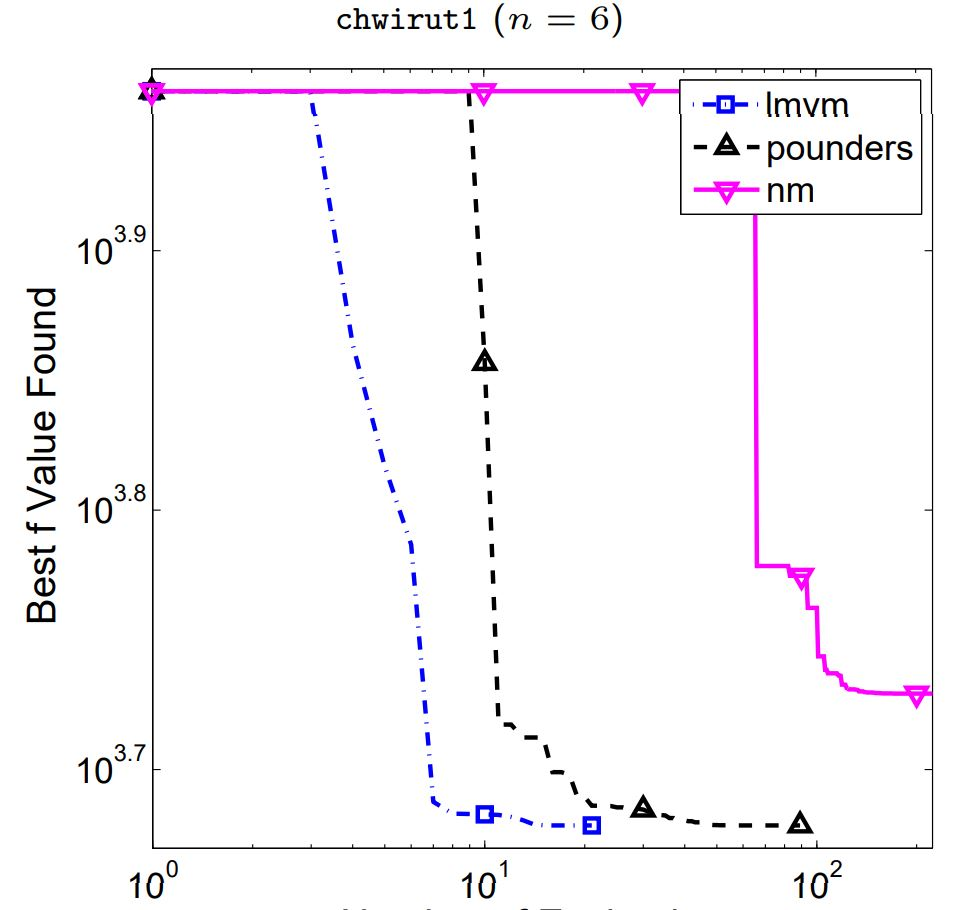
\includegraphics[width=\textwidth]{fig/8.jpg}
\begin{center}
Number of Evaluations
\end{center}

\column{0.5\textwidth}
\flushright{
\scriptsize{
Toolkit for Advanced Optimization\\
\textcolor[RGB]{128,0,128}{[Munson et al.; mcs.anl.gov/tao]}
}
}
\colorbox[rgb]{0.5,0.6,0.7}{\textcolor{white}{Increasing level of user input:}}

\begin{table}[]\scriptsize
\begin{tabular}{rl}
\textbf{\textcolor[RGB]{128,0,128}{nm}} & Assumes $\nabla_x f$\\
										& unavailable,\textcolor{red}{black box} \\
\textbf{pounders} 						& Assumes $\nabla_x f$\\
										& unavailable,\textcolor{blue}{exploits}\\
										& \textcolor{blue}{problem structure}\\
										& $\qquad\qquad$\textcolor{blue}{THIS TALK}\\
\textbf{\textcolor{blue}{lmvm}}     	& Uses available $\nabla_x f$
\end{tabular}
\end{table}

\emph{DFO methods should be designed to beat finite-difference-based methods}
\end{columns}

\vspace{0.2cm} 
\textcolor{blue}{Observe:}Constrained by budget on $\#$evals, method limits solution accuracy/problem size
\end{frame}

%9-1
\begin{frame}{Global Optimization, $\textup{min}_{x\in\Omega} f(x)$}
Careful:
\begin{itemize}
\small{
\item \textcolor{blue}{Global convergence}:Convergence (to a local solution/stationary point) from anywhere in $\Omega$
\item \textcolor{blue}{Convergence to a global minimizer}:Obtain $x^*$ with $f(x^*)\le f(x)\forall x\in\Omega$
}
\end{itemize}

\rule{\textwidth}{1pt}
\vspace{4.5cm}
\end{frame}

%9-2
\begin{frame}{Global Optimization, $\textup{min}_{x\in\Omega} f(x)$}
Careful:
\begin{itemize}
\small{
\item \textcolor{blue}{Global convergence}:Convergence (to a local solution/stationary point) from anywhere in $\Omega$
\item \textcolor{blue}{Convergence to a global minimizer}:Obtain $x^*$ with $f(x^*)\le f(x)\forall x\in\Omega$
}
\end{itemize}

\rule{\textwidth}{1pt}
\footnotesize{
\textbf{Anyone selling you global solutions when derivatives are unavailable:}
}
\begin{table}[]\scriptsize
\begin{tabular}{rll}
\textcolor{red}{either}   & \multicolumn{2}{l}{assumes more about your problem (e.g., convex $f$)}\\
\textcolor{red}{or} & \multicolumn{2}{l}{expects you to wait forever} \\
 & \textcolor{cyan}{T$\ddot{\textup{o}}$rn and $\breve{\textup{Z}}$ilinskas:} & An algorithm converges to the global minimum for any \\
         &                      & continuous $f$ if and only if the sequence of points visited  \\
   &            & by the algorithm is dense in $\Omega$.\\
\textcolor{red}{or} & \multicolumn{2}{l}{cannot be trusted}          
\end{tabular}
\end{table}

\rule{\textwidth}{1pt}
\vspace{1.4cm} 
\end{frame}

%9-3
\begin{frame}{Global Optimization, $\textup{min}_{x\in\Omega} f(x)$}
Careful:
\begin{itemize}
\small{
\item \textcolor{blue}{Global convergence}:Convergence (to a local solution/stationary point) from anywhere in $\Omega$
\item \textcolor{blue}{Convergence to a global minimizer}:Obtain $x^*$ with $f(x^*)\le f(x)\forall x\in\Omega$
}
\end{itemize}

\rule{\textwidth}{1pt}
\footnotesize{
\textbf{Anyone selling you global solutions when derivatives are unavailable:}
}
\begin{table}[]\scriptsize
\begin{tabular}{rll}
\textcolor{red}{either}   & \multicolumn{2}{l}{assumes more about your problem (e.g., convex $f$)}\\
\textcolor{red}{or} & \multicolumn{2}{l}{expects you to wait forever} \\
 & \textcolor{cyan}{T$\ddot{\textup{o}}$rn and $\breve{\textup{Z}}$ilinskas:} & An algorithm converges to the global minimum for any \\
         &                      & continuous $f$ if and only if the sequence of points visited  \\
   &            & by the algorithm is dense in $\Omega$.\\
\textcolor{red}{or} & \multicolumn{2}{l}{cannot be trusted}          
\end{tabular}
\end{table}

\rule{\textwidth}{1pt}
Instead:
\begin{itemize}
\small{
\item Rapidly find good local solutions and/or be robust to poor solutions
\item Consider multistart approaches and/or structure of multimodality
}
\end{itemize}
\end{frame}

%10
\begin{frame}{(One Reason) Why We Won’t Be Talking About Heuristics}
\begin{center}
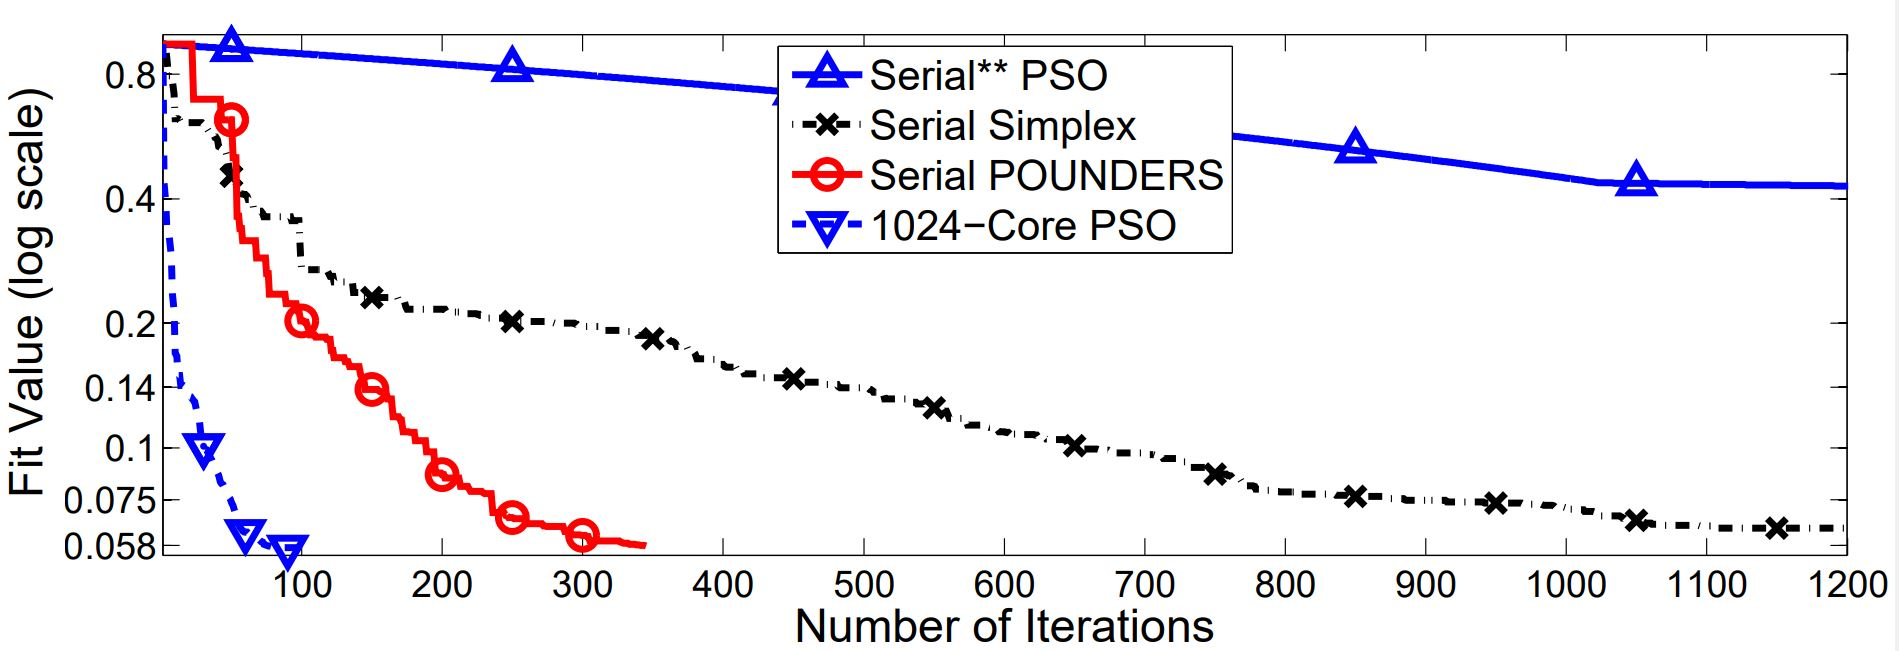
\includegraphics[width=0.9\textwidth]{fig/10.jpg}
\end{center}

\begin{itemize}\scriptsize
\item Heuristics often “embarrassingly/naturally parallel”;\\
\textcolor{blue}{PSO}= particle swarm method
	\begin{itemize}\scriptsize
	\item Typically through stochastic sampling/evolution
	\item 1024 function evaluations per iteration
	\end{itemize}
\item \textcolor{blue}{Simplex} is Nelder-Mead; \textcolor{blue}{POUNDERS} is model-based\\
trust-region algorithm
	\begin{itemize}\scriptsize
	\item one function evaluation per iteration
	\end{itemize}
\item [\textcolor{red}{$\rightarrow$}] Is this an effective use of resources?
\item [\textcolor{red}{$\rightarrow$}] How many cores would have sufficed?
\end{itemize}
\end{frame}

%section1
\section{Black-Box Optimization}

%12-1
\begin{frame}{Black-box Optimization Problems}
\begin{columns}
\column{0.35\textwidth}
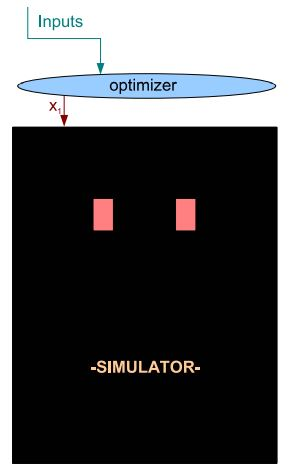
\includegraphics[width=\textwidth]{fig/12-1.jpg}

\column{0.65\textwidth}
\small{
\colorbox[rgb]{0.5,0.6,0.7}{\textcolor{white}{Only knowledge about $f$ is obtained by sampling}}
}
\begin{itemize}\small
\item $f=S$\;a black box (running some executable-only code or performing an experiment in the lab)
\item Only give a single output (no derivatives $\nabla_x S(x)$)
\end{itemize}

\small{
\colorbox[rgb]{0.5,0.6,0.7}{\textcolor{white}{Good solutions guaranteed in the limit, but:}}
}
\begin{itemize}\small
\item Usually have \underline{computational budget} (due to scheduling,finances, deadlines)
\item Limited number of evaluations
\end{itemize}
\end{columns}
\end{frame}

%12-2
\begin{frame}{Black-box Optimization Problems}
\begin{columns}
\column{0.35\textwidth}
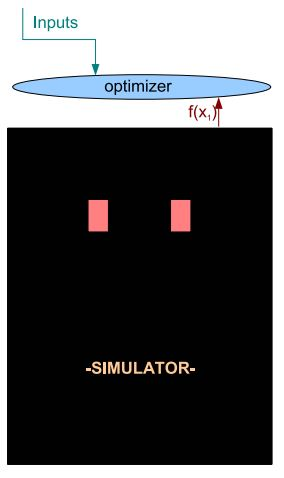
\includegraphics[width=\textwidth]{fig/12-2.jpg}

\column{0.65\textwidth}
\small{
\colorbox[rgb]{0.5,0.6,0.7}{\textcolor{white}{Only knowledge about $f$ is obtained by sampling}}
}
\begin{itemize}\small
\item $f=S$\;a black box (running some executable-only code or performing an experiment in the lab)
\item Only give a single output (no derivatives $\nabla_x S(x)$)
\end{itemize}

\small{
\colorbox[rgb]{0.5,0.6,0.7}{\textcolor{white}{Good solutions guaranteed in the limit, but:}}
}
\begin{itemize}\small
\item Usually have \underline{computational budget} (due to scheduling,finances, deadlines)
\item Limited number of evaluations
\end{itemize}
\end{columns}
\end{frame}

%13
\begin{frame}{A Black Box: Automating Empirical Performance Tuning}
\begin{columns}
\column{0.5\textwidth}
Given semantically equivalent codes $x^1,x^2,...$, minimize run time subject to energy consumption
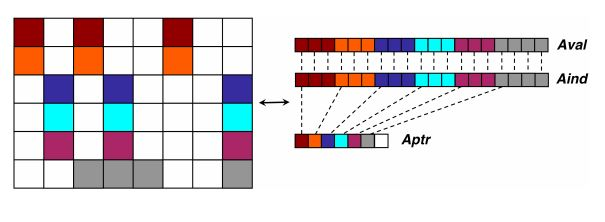
\includegraphics[width=\textwidth]{fig/13-1.jpg}

\column{0.5\textwidth}
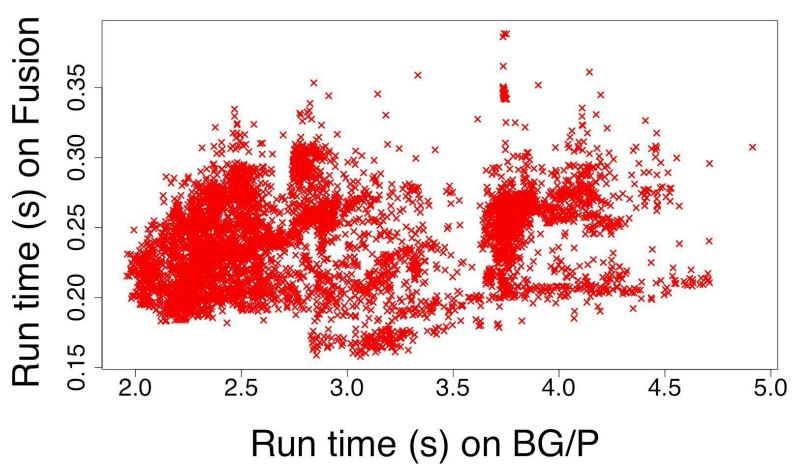
\includegraphics[width=\textwidth]{fig/13-2.jpg}
\end{columns}

\colorbox[rgb]{0.5,0.6,0.7}{\textcolor{white}{$\min\{f(x):(x_C,x_I,x_B)\in\Omega_C\times\Omega_I\times\Omega_B\}$}}
\begin{itemize}
\item [\textcolor{blue}{$x$}] multidimensional parameterization (compiler type, compiler flags, unroll/tiling factors, internal tolerances, . . . )
\item [\textcolor{blue}{$\Omega$}] search domain (feasible transformation, no errors)
\item [\textcolor{blue}{$f$}] quantifiable performance objective (requires a run)
\end{itemize}

\flushright{
\tiny{
\textcolor{blue}{$\rightarrow$}
\textcolor[RGB]{128,0,128}{[Audet \& Orban; SIOPT 2006], [Balaprakash, W., Hovland; ICCS 2011], [Porcelli \& Toint; 2016]}\\
Numerical Linear Algebra
\textcolor{blue}{$\rightarrow$}
\textcolor[RGB]{128,0,128}{[N. Higham; SIMAX 1993]}
,...
}
}
\end{frame}

%14
\begin{frame}{Optimization for Automatic Tuning of HPC Codes}
Evaluation of $f$ requires:

transforming source, compilation, (repeated?) execution, checking for correctness

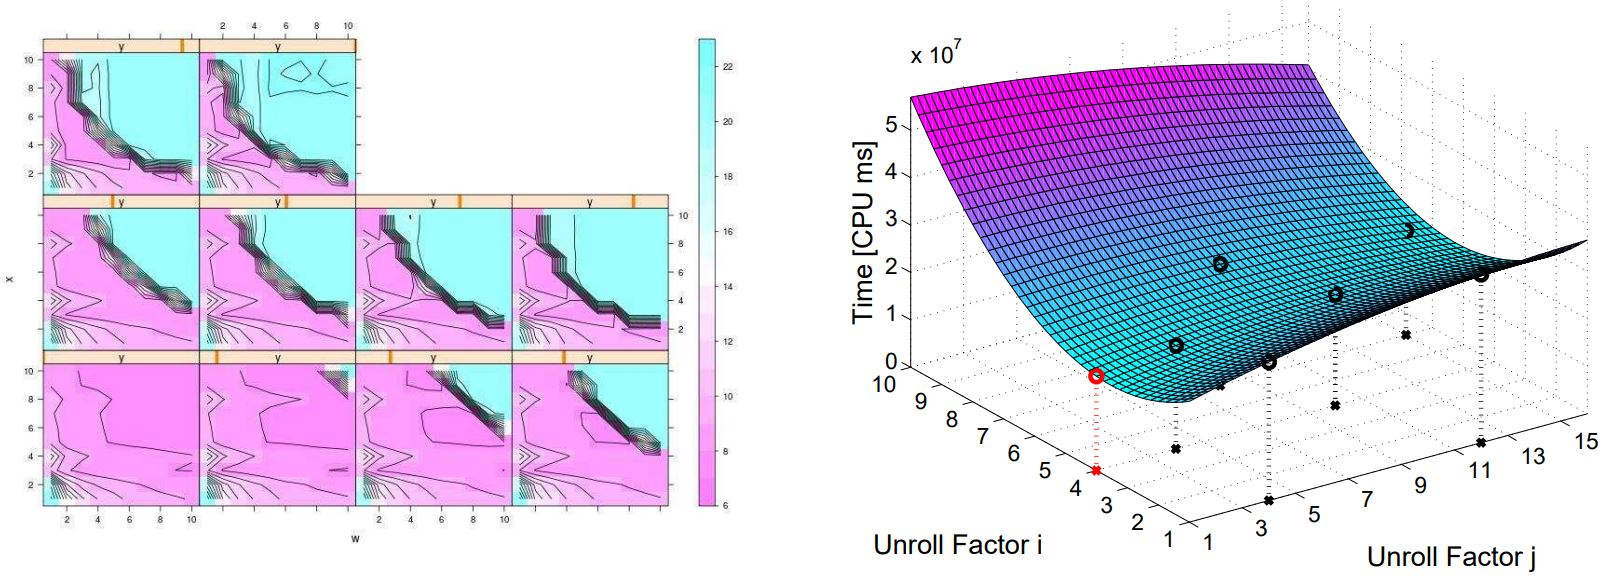
\includegraphics[width=\textwidth]{fig/14.jpg}

\rule{\textwidth}{1pt}

\textcolor{red}{Challenges:}

\begin{columns}
\column{0.5\textwidth}
\begin{itemize}\scriptsize
\item [\textcolor{red}{-}] Evaluating $f(\Omega)$ prohibitively expensive (e.g., $10^{19}$ discrete decisions)
\item [\textcolor{red}{-}] $f$\;noisy
\end{itemize}

\column{0.5\textwidth}
\begin{itemize}\scriptsize
\item [\textcolor{red}{-}] Discrete $x$ unrelaxable
\item [\textcolor{red}{-}] $\nabla_x f$ unavailable/nonexistent
\item [\textcolor{red}{-}] Many distinct/local solutions
\end{itemize}
\end{columns}
\end{frame}

%15
\begin{frame}{Black-box Algorithms}
\colorbox[rgb]{0.5,0.6,0.7}{\textcolor{white}{Solve general problems $\min\{f(x):x\in \mathbb{R}^n\}$:}}
\begin{itemize}
\item Only require function values (no $\nabla f(x)$)
\item  Don't rely on finite-difference approximations to $\nabla f(x)$
\item Seek greedy and rapid decrease of function value
\item Have asymptotic convergence guarantees
\item  Assume parallel resources are used \underline{within} function evaluation
\end{itemize}

\colorbox[rgb]{0.5,0.6,0.7}{\textcolor{white}{Main styles of DFO algorithms}}
\begin{itemize}
\item Randomized methods (later?)
\item Direct search methods (pattern search, Nelder-Mead, . . . )
\item Model-based methods (quadratics, radial basis functions, . . .) 
\end{itemize}
\end{frame}

%16-1
\begin{frame}{Black-Box Algorithms: Stochastic Methods}
\colorbox[rgb]{0.5,0.6,0.7}{\textcolor{white}{Random search}}

Repeat:
\begin{enumerate}
\item Randomly generate direction $d^k\in\mathbb{R}^n$
\item  Evaluate “gradient-free oracle” $g(x^k;h_k)=\frac{\textcolor{red}{f(x^k+h_kd^k)}-f(x^k)}{h_k}d^k$

$\qquad\qquad\qquad\qquad\qquad\qquad\qquad\qquad$ ($\textcolor{blue}{\approx }$ \textcolor{blue}{directional derivative})

\item Compute $x^{k+1}=x^k-\delta_k g(x^k;h_k)$, evaluate $\textcolor{red}{f(x^{k+1})}$
\end{enumerate}
Convergence (for different types of $f$) tends to be probabilistic

\scriptsize
\textcolor[RGB]{128,0,128}{[[Kiefer \& Wolfowitz; AnnMS 1952], [\underline{Polyak}; 1987], [Ghadimi \& Lan; SIOPT 2013], [Nesterov \& Spokoiny; FoCM 2015], . . .}

\vspace{2.5cm}
\end{frame}

%16-2
\begin{frame}{Black-Box Algorithms: Stochastic Methods}
\colorbox[rgb]{0.5,0.6,0.7}{\textcolor{white}{Random search}}

Repeat:
\begin{enumerate}
\item Randomly generate direction $d^k\in\mathbb{R}^n$
\item  Evaluate “gradient-free oracle” $g(x^k;h_k)=\frac{\textcolor{red}{f(x^k+h_kd^k)}-f(x^k)}{h_k}d^k$

$\qquad\qquad\qquad\qquad\qquad\qquad\qquad\qquad$ ($\textcolor{blue}{\approx }$ \textcolor{blue}{directional derivative})

\item Compute $x^{k+1}=x^k-\delta_k g(x^k;h_k)$, evaluate $\textcolor{red}{f(x^{k+1})}$
\end{enumerate}
Convergence (for different types of $f$) tends to be probabilistic

\scriptsize
\textcolor[RGB]{128,0,128}{[[Kiefer \& Wolfowitz; AnnMS 1952], [\underline{Polyak}; 1987], [Ghadimi \& Lan; SIOPT 2013], [Nesterov \& Spokoiny; FoCM 2015], . . .}

\normalsize
\colorbox[rgb]{0.5,0.6,0.7}{\textcolor{white}{Stochastic heuristics (nature-inspired methods, etc.)}}

\begin{itemize}
\item Popular in practice, especially in engineering
\item Typically global in nature
\item \textcolor{red}{Require many $f$ evaluations}
\end{itemize}
\end{frame}

%subsection
\subsection{Direct Search Methods}

%17-1
\begin{frame}{Pattern Search And Its Variants}\footnotesize
Choose a set of directions (\textcolor{blue}{pattern} or \textcolor{blue}{mesh}) $\mathcal{D}^k$

\begin{itemize}
\item[\textcolor{cyan}{Ex.-}] $\pm$ coordinate directions ($2n$ directions)
\item[\textcolor{cyan}{Ex.-}] any minimal positive spanning set ([$e_1,...e_n,-\sum e_i$])
\end{itemize}

\begin{columns}
\column{0.5\textwidth}
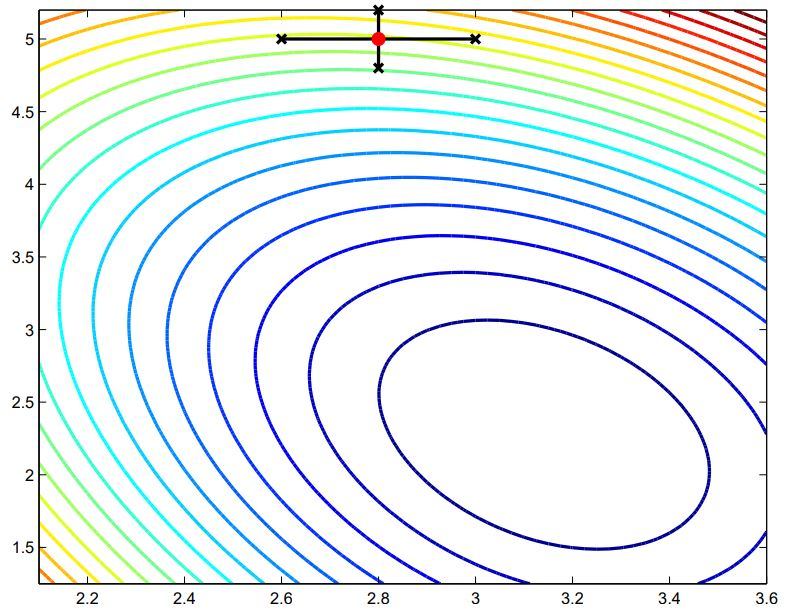
\includegraphics[width=\textwidth]{fig/17-1.jpg}

\column{0.5\textwidth}
\colorbox[rgb]{0.5,0.6,0.7}{\textcolor{white}{Basic iteration($k\ge0$):}}
\begin{itemize}\scriptsize
\item Evaluate $f(x^k+\Delta_kd^j),j=1,...,|\mathcal{D}^k|$
\item If $[f(x^k+\Delta_kd^j)<f(x^k)]$, 

$\quad$move to $x^{k+1}=x^k+\Delta_kd^j$\\

Otherwise shrink$\Delta_k$
\item Update$\mathcal{D}^k$
\end{itemize}
This is an \textcolor{blue}{indicator} function, does not say anything about the magnitude of $f$ values, just the ordering
\end{columns}

\vspace{1.2cm}

\tiny
\flushright{Suivey$\textcolor{blue}{\rightarrow}$\textcolor[RGB]{128,0,128}{[Kolda, Lewis, Torczon; SIREV 2003]}}

\flushright{Tools$\textcolor{blue}{\rightarrow}$ DFL\textcolor[RGB]{128,0,128}{[Liuzzi et al.]}, NOMAD\textcolor[RGB]{128,0,128}{[Audet et al.]}, . . .}
\end{frame}

%17-2
\begin{frame}{Pattern Search And Its Variants}\footnotesize
Choose a set of directions (\textcolor{blue}{pattern} or \textcolor{blue}{mesh}) $\mathcal{D}^k$

\begin{itemize}
\item[\textcolor{cyan}{Ex.-}] $\pm$ coordinate directions ($2n$ directions)
\item[\textcolor{cyan}{Ex.-}] any minimal positive spanning set ([$e_1,...e_n,-\sum e_i$])
\end{itemize}

\begin{columns}
\column{0.5\textwidth}
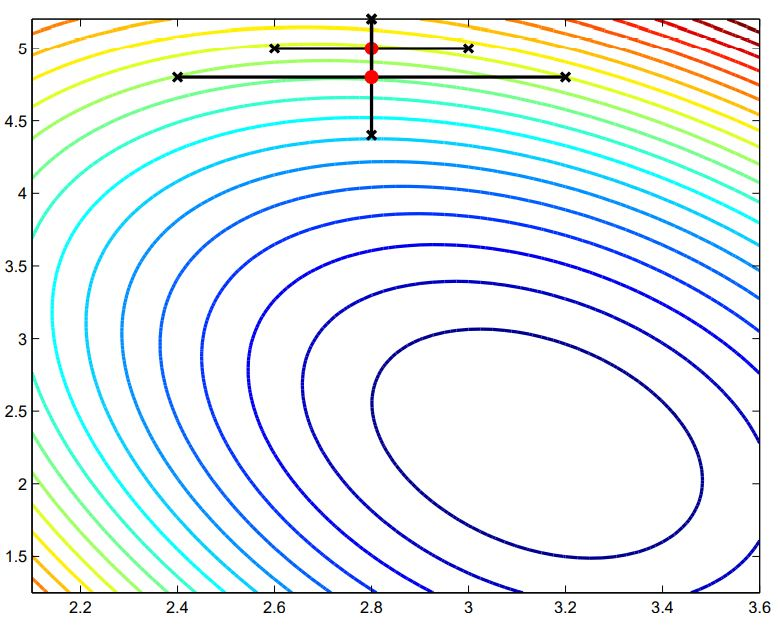
\includegraphics[width=\textwidth]{fig/17-2.jpg}

\column{0.5\textwidth}
\colorbox[rgb]{0.5,0.6,0.7}{\textcolor{white}{Basic iteration($k\ge0$):}}
\begin{itemize}\scriptsize
\item Evaluate $f(x^k+\Delta_kd^j),j=1,...,|\mathcal{D}^k|
$\item If $[f(x^k+\Delta_kd^j)<f(x^k)]$, 

$\quad$move to $x^{k+1}=x^k+\Delta_kd^j$\\

Otherwise shrink$\Delta_k$
\item Update$\mathcal{D}^k$
\end{itemize}
This is an \textcolor{blue}{indicator} function, does not say anything about the magnitude of $f$ values, just the ordering
\end{columns}

\vspace{1.2cm}

\tiny
\flushright{Suivey$\textcolor{blue}{\rightarrow}$\textcolor[RGB]{128,0,128}{[Kolda, Lewis, Torczon; SIREV 2003]}}

\flushright{Tools$\textcolor{blue}{\rightarrow}$ DFL\textcolor[RGB]{128,0,128}{[Liuzzi et al.]}, NOMAD\textcolor[RGB]{128,0,128}{[Audet et al.]}, . . .}
\end{frame}

%17-3
\begin{frame}{Pattern Search And Its Variants}\footnotesize
Choose a set of directions (\textcolor{blue}{pattern} or \textcolor{blue}{mesh}) $\mathcal{D}^k$

\begin{itemize}
\item[\textcolor{cyan}{Ex.-}] $\pm$ coordinate directions ($2n$ directions)
\item[\textcolor{cyan}{Ex.-}] any minimal positive spanning set ([$e_1,...e_n,-\sum e_i$])
\end{itemize}

\begin{columns}
\column{0.5\textwidth}
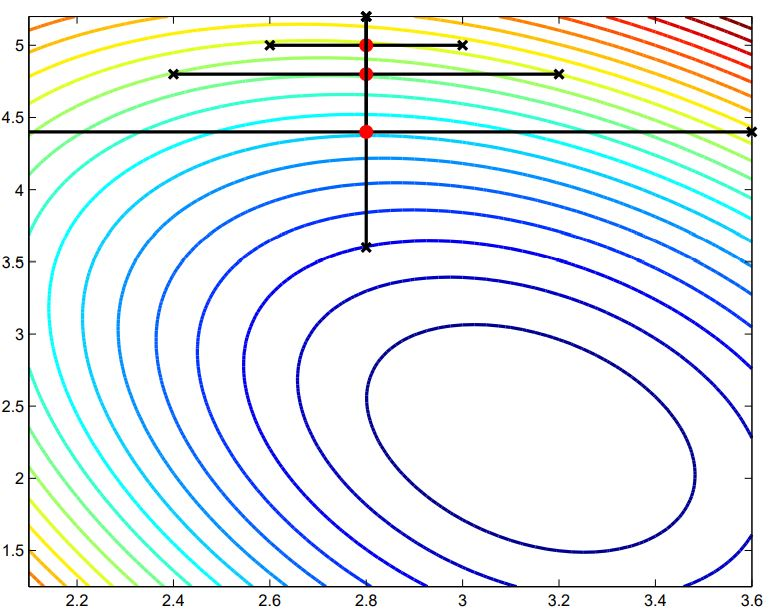
\includegraphics[width=\textwidth]{fig/17-3.jpg}

\column{0.5\textwidth}
\colorbox[rgb]{0.5,0.6,0.7}{\textcolor{white}{Basic iteration($k\ge0$):}}
\begin{itemize}\scriptsize
\item Evaluate $f(x^k+\Delta_kd^j),j=1,...,|\mathcal{D}^k|$
\item If $[f(x^k+\Delta_kd^j)<f(x^k)]$, 

$\quad$move to $x^{k+1}=x^k+\Delta_kd^j$\\

Otherwise shrink$\Delta_k$
\item Update$\mathcal{D}^k$
\end{itemize}
This is an \textcolor{blue}{indicator} function, does not say anything about the magnitude of $f$ values, just the ordering
\end{columns}

\vspace{1.2cm}

\tiny
\flushright{Suivey$\textcolor{blue}{\rightarrow}$\textcolor[RGB]{128,0,128}{[Kolda, Lewis, Torczon; SIREV 2003]}}

\flushright{Tools$\textcolor{blue}{\rightarrow}$ DFL\textcolor[RGB]{128,0,128}{[Liuzzi et al.]}, NOMAD\textcolor[RGB]{128,0,128}{[Audet et al.]}, . . .}
\end{frame}

%17-4
\begin{frame}{Pattern Search And Its Variants}\footnotesize
Choose a set of directions (\textcolor{blue}{pattern} or \textcolor{blue}{mesh}) $\mathcal{D}^k$

\begin{itemize}
\item[\textcolor{cyan}{Ex.-}] $\pm$ coordinate directions ($2n$ directions)
\item[\textcolor{cyan}{Ex.-}] any minimal positive spanning set ([$e_1,...e_n,-\sum e_i$])
\end{itemize}

\begin{columns}
\column{0.5\textwidth}
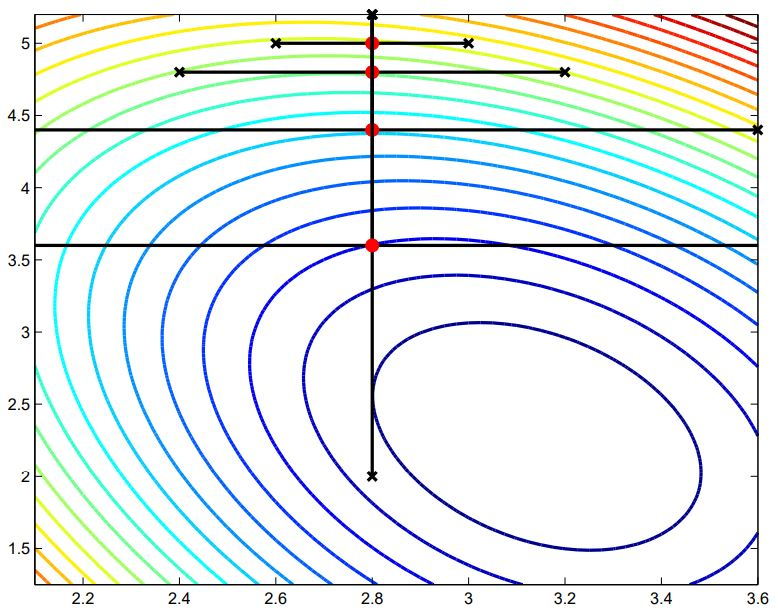
\includegraphics[width=\textwidth]{fig/17-4.jpg}

\column{0.5\textwidth}
\colorbox[rgb]{0.5,0.6,0.7}{\textcolor{white}{Basic iteration($k\ge0$):}}
\begin{itemize}\scriptsize
\item Evaluate $f(x^k+\Delta_kd^j),j=1,...,|\mathcal{D}^k|$
\item If $[f(x^k+\Delta_kd^j)<f(x^k)]$, 

$\quad$move to $x^{k+1}=x^k+\Delta_kd^j$\\

Otherwise shrink$\Delta_k$
\item Update$\mathcal{D}^k$
\end{itemize}
This is an \textcolor{blue}{indicator} function, does not say anything about the magnitude of $f$ values, just the ordering
\end{columns}

\vspace{1.2cm}

\tiny
\flushright{Suivey$\textcolor{blue}{\rightarrow}$\textcolor[RGB]{128,0,128}{[Kolda, Lewis, Torczon; SIREV 2003]}}

\flushright{Tools$\textcolor{blue}{\rightarrow}$ DFL\textcolor[RGB]{128,0,128}{[Liuzzi et al.]}, NOMAD\textcolor[RGB]{128,0,128}{[Audet et al.]}, . . .}
\end{frame}

%17-5
\begin{frame}{Pattern Search And Its Variants}\footnotesize
Choose a set of directions (\textcolor{blue}{pattern} or \textcolor{blue}{mesh}) $\mathcal{D}^k$

\begin{itemize}
\item[\textcolor{cyan}{Ex.-}] $\pm$ coordinate directions ($2n$ directions)
\item[\textcolor{cyan}{Ex.-}] any minimal positive spanning set ([$e_1,...e_n,-\sum e_i$])
\end{itemize}

\begin{columns}
\column{0.5\textwidth}
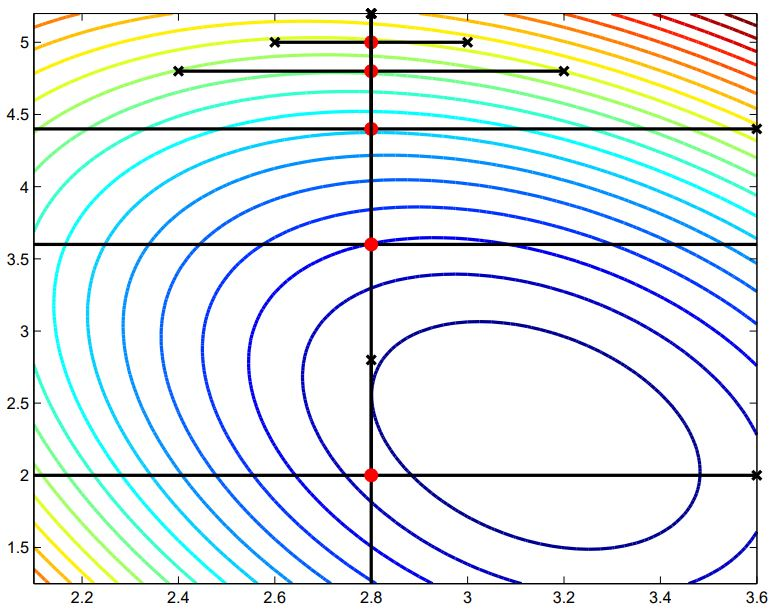
\includegraphics[width=\textwidth]{fig/17-5.jpg}

\column{0.5\textwidth}
\colorbox[rgb]{0.5,0.6,0.7}{\textcolor{white}{Basic iteration($k\ge0$):}}
\begin{itemize}\scriptsize
\item Evaluate $f(x^k+\Delta_kd^j),j=1,...,|\mathcal{D}^k|$
\item If $[f(x^k+\Delta_kd^j)<f(x^k)]$, 

$\quad$move to $x^{k+1}=x^k+\Delta_kd^j$\\

Otherwise shrink$\Delta_k$
\item Update$\mathcal{D}^k$
\end{itemize}
This is an \textcolor{blue}{indicator} function, does not say anything about the magnitude of $f$ values, just the ordering
\end{columns}

\vspace{1.2cm}

\tiny
\flushright{Suivey$\textcolor{blue}{\rightarrow}$\textcolor[RGB]{128,0,128}{[Kolda, Lewis, Torczon; SIREV 2003]}}

\flushright{Tools$\textcolor{blue}{\rightarrow}$ DFL\textcolor[RGB]{128,0,128}{[Liuzzi et al.]}, NOMAD\textcolor[RGB]{128,0,128}{[Audet et al.]}, . . .}
\end{frame}

%17-6
\begin{frame}{Pattern Search And Its Variants}\footnotesize
Choose a set of directions (\textcolor{blue}{pattern} or \textcolor{blue}{mesh}) $\mathcal{D}^k$

\begin{itemize}
\item[\textcolor{cyan}{Ex.-}] $\pm$ coordinate directions ($2n$ directions)
\item[\textcolor{cyan}{Ex.-}] any minimal positive spanning set ([$e_1,...e_n,-\sum e_i$])
\end{itemize}

\begin{columns}
\column{0.5\textwidth}
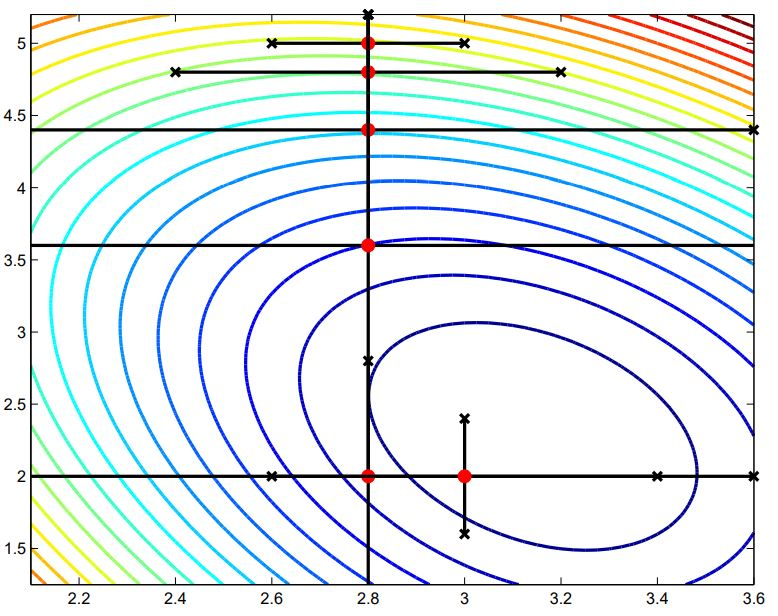
\includegraphics[width=\textwidth]{fig/17-6.jpg}

\column{0.5\textwidth}
\colorbox[rgb]{0.5,0.6,0.7}{\textcolor{white}{Basic iteration($k\ge0$):}}
\begin{itemize}\scriptsize
\item Evaluate $f(x^k+\Delta_kd^j),j=1,...,|\mathcal{D}^k|$
\item If $[f(x^k+\Delta_kd^j)<f(x^k)]$, 

$\quad$move to $x^{k+1}=x^k+\Delta_kd^j$\\

Otherwise shrink$\Delta_k$
\item Update$\mathcal{D}^k$
\end{itemize}
This is an \textcolor{blue}{indicator} function, does not say anything about the magnitude of $f$ values, just the ordering
\end{columns}

\vspace{1.2cm}

\tiny
\flushright{Suivey$\textcolor{blue}{\rightarrow}$\textcolor[RGB]{128,0,128}{[Kolda, Lewis, Torczon; SIREV 2003]}}

\flushright{Tools$\textcolor{blue}{\rightarrow}$ DFL\textcolor[RGB]{128,0,128}{[Liuzzi et al.]}, NOMAD\textcolor[RGB]{128,0,128}{[Audet et al.]}, . . .}
\end{frame}

%17-7
\begin{frame}{Pattern Search And Its Variants}\footnotesize
Choose a set of directions (\textcolor{blue}{pattern} or \textcolor{blue}{mesh}) $\mathcal{D}^k$

\begin{itemize}
\item[\textcolor{cyan}{Ex.-}] $\pm$ coordinate directions ($2n$ directions)
\item[\textcolor{cyan}{Ex.-}] any minimal positive spanning set ([$e_1,...e_n,-\sum e_i$])
\end{itemize}

\begin{columns}
\column{0.5\textwidth}
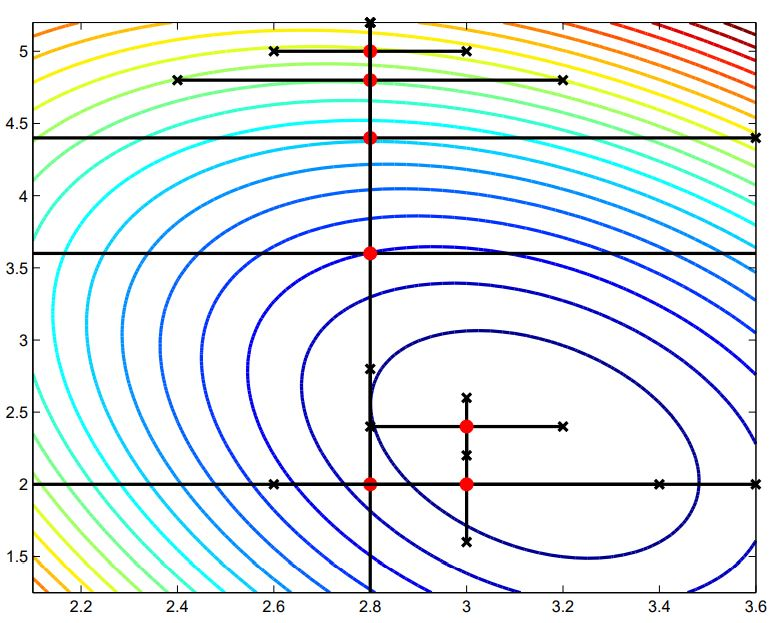
\includegraphics[width=\textwidth]{fig/17-7.jpg}

\column{0.5\textwidth}
\colorbox[rgb]{0.5,0.6,0.7}{\textcolor{white}{Basic iteration($k\ge0$):}}
\begin{itemize}\scriptsize
\item Evaluate $f(x^k+\Delta_kd^j),j=1,...,|\mathcal{D}^k|$
\item If $[f(x^k+\Delta_kd^j)<f(x^k)]$, 

$\quad$move to $x^{k+1}=x^k+\Delta_kd^j$\\

Otherwise shrink$\Delta_k$
\item Update$\mathcal{D}^k$
\end{itemize}
This is an \textcolor{blue}{indicator} function, does not say anything about the magnitude of $f$ values, just the ordering
\end{columns}

\begin{itemize}\scriptsize
\item[$\textcolor{blue}{\rightarrow }$] Lends itself well to doing concurrent function evaluations
\item[$\textcolor{blue}{\rightarrow }$] See also mesh-adaptive direct search methods
\item[$\textcolor{blue}{\rightarrow }$] Can establish convergence for nonsmooth $f$
\end{itemize}

\tiny
\flushright{Suivey$\textcolor{blue}{\rightarrow}$\textcolor[RGB]{128,0,128}{[Kolda, Lewis, Torczon; SIREV 2003]}}

\flushright{Tools$\textcolor{blue}{\rightarrow}$ DFL\textcolor[RGB]{128,0,128}{[Liuzzi et al.]}, NOMAD\textcolor[RGB]{128,0,128}{[Audet et al.]}, . . .}
\end{frame}

%18-1
\begin{frame}{The Nelder-Mead Method [1965]}
\begin{columns}
\column{0.43\textwidth}
\colorbox[rgb]{0.5,0.6,0.7}{\textcolor{white}{Basic iteration($k\ge0$):}}
\begin{itemize}\footnotesize
\item Evaluate $f$\,on the $n+1$\,vertices of the simplex\,$x^k+\Delta_kS^{(k)}$
\item Reflect worst vertex about the best face
\item Shrink, contract, or expand\,$\Delta_kS^{(k)}$
\end{itemize}

\column{0.57\textwidth}
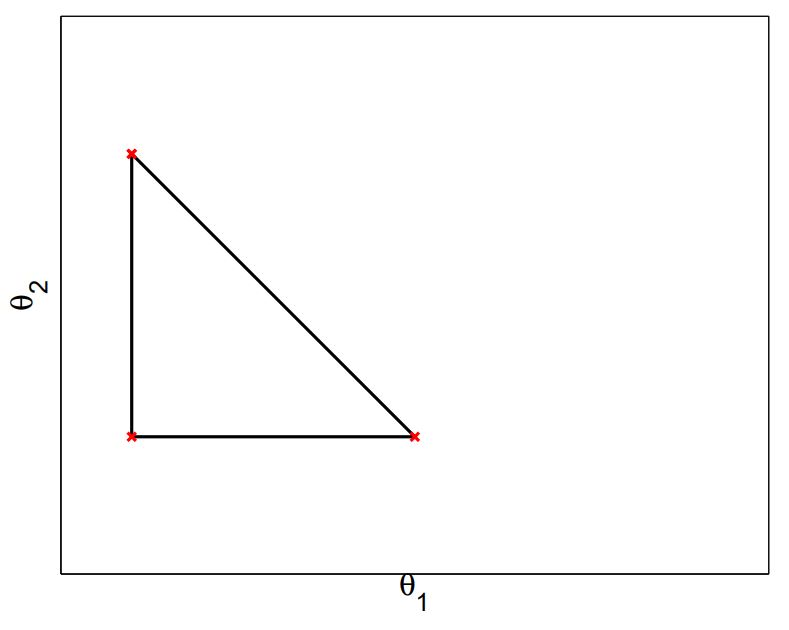
\includegraphics[width=\textwidth]{fig/18-1.jpg}
\end{columns}

\vspace{2.4cm}
\end{frame}

%18-2
\begin{frame}{The Nelder-Mead Method [1965]}
\begin{columns}
\column{0.43\textwidth}
\colorbox[rgb]{0.5,0.6,0.7}{\textcolor{white}{Basic iteration($k\ge0$):}}
\begin{itemize}\footnotesize
\item Evaluate $f$\,on the $n+1$\,vertices of the simplex\,$x^k+\Delta_kS^{(k)}$
\item Reflect worst vertex about the best face
\item Shrink, contract, or expand\,$\Delta_kS^{(k)}$
\end{itemize}

\column{0.57\textwidth}
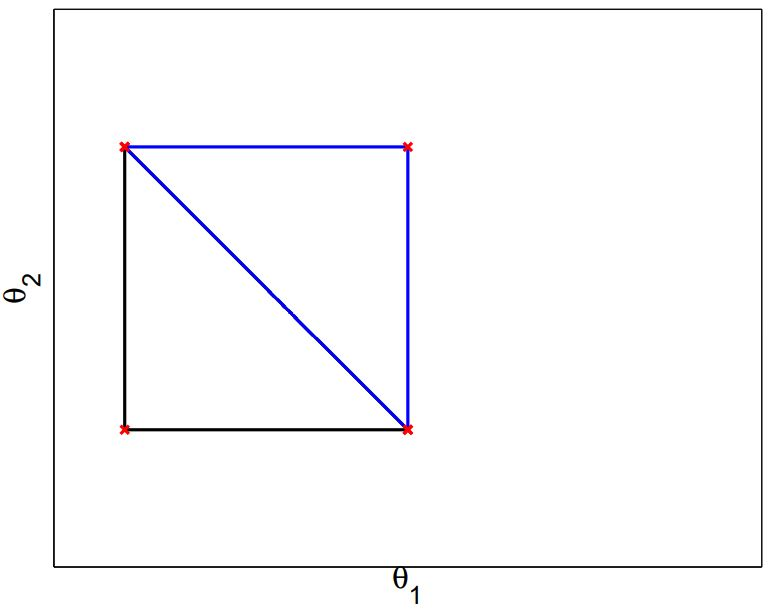
\includegraphics[width=\textwidth]{fig/18-2.jpg}
\end{columns}

\vspace{2.4cm}
\end{frame}

%18-3
\begin{frame}{The Nelder-Mead Method [1965]}
\begin{columns}
\column{0.43\textwidth}
\colorbox[rgb]{0.5,0.6,0.7}{\textcolor{white}{Basic iteration($k\ge0$):}}
\begin{itemize}\footnotesize
\item Evaluate $f$\,on the $n+1$\,vertices of the simplex\,$x^k+\Delta_kS^{(k)}$
\item Reflect worst vertex about the best face
\item Shrink, contract, or expand\,$\Delta_kS^{(k)}$
\end{itemize}

\column{0.57\textwidth}
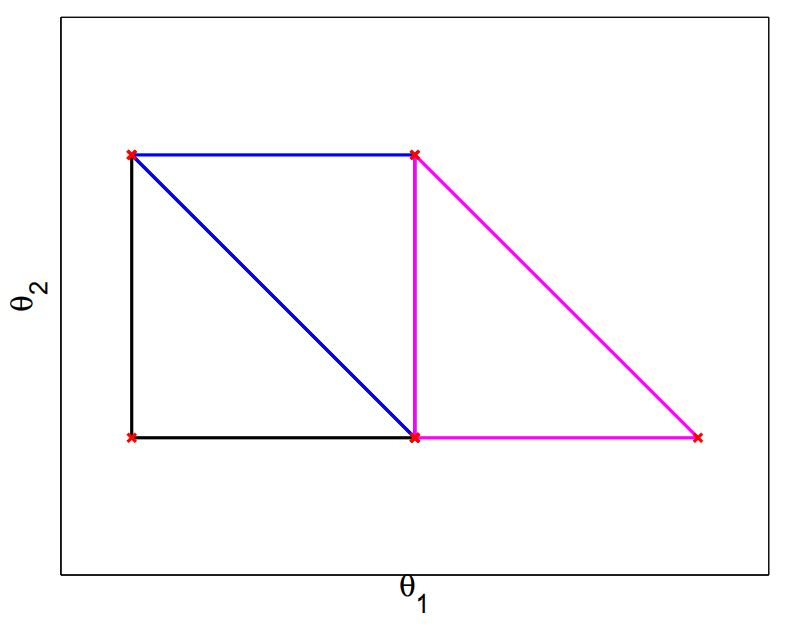
\includegraphics[width=\textwidth]{fig/18-3.jpg}
\end{columns}

\vspace{2.4cm}
\end{frame}

%18-4
\begin{frame}{The Nelder-Mead Method [1965]}
\begin{columns}
\column{0.43\textwidth}
\colorbox[rgb]{0.5,0.6,0.7}{\textcolor{white}{Basic iteration($k\ge0$):}}
\begin{itemize}\footnotesize
\item Evaluate $f$\,on the $n+1$\,vertices of the simplex\,$x^k+\Delta_kS^{(k)}$
\item Reflect worst vertex about the best face
\item Shrink, contract, or expand\,$\Delta_kS^{(k)}$
\end{itemize}

\column{0.57\textwidth}
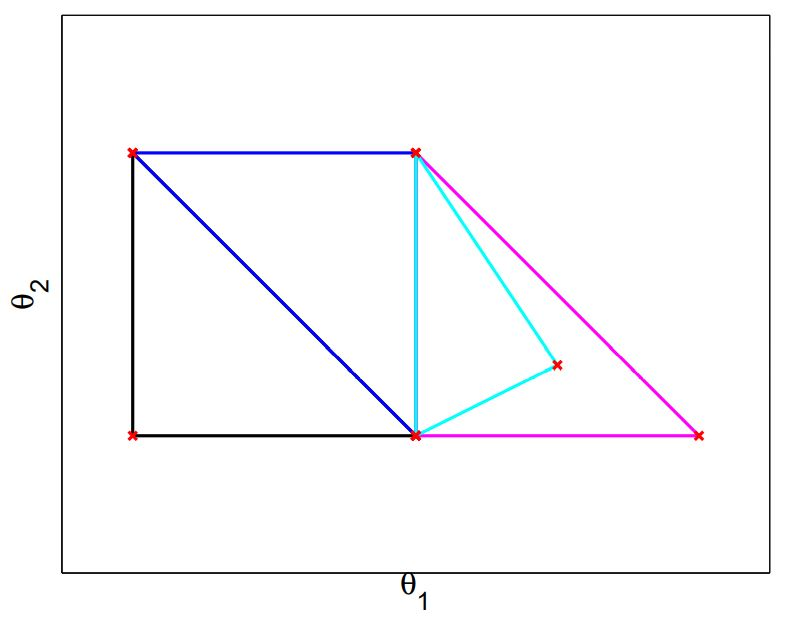
\includegraphics[width=\textwidth]{fig/18-4.jpg}
\end{columns}

\vspace{2.4cm}
\end{frame}

%18-5
\begin{frame}{The Nelder-Mead Method [1965]}
\begin{columns}
\column{0.43\textwidth}
\colorbox[rgb]{0.5,0.6,0.7}{\textcolor{white}{Basic iteration($k\ge0$):}}
\begin{itemize}\footnotesize
\item Evaluate $f$\,on the $n+1$\,vertices of the simplex\,$x^k+\Delta_kS^{(k)}$
\item Reflect worst vertex about the best face
\item Shrink, contract, or expand\,$\Delta_kS^{(k)}$
\end{itemize}

\column{0.57\textwidth}
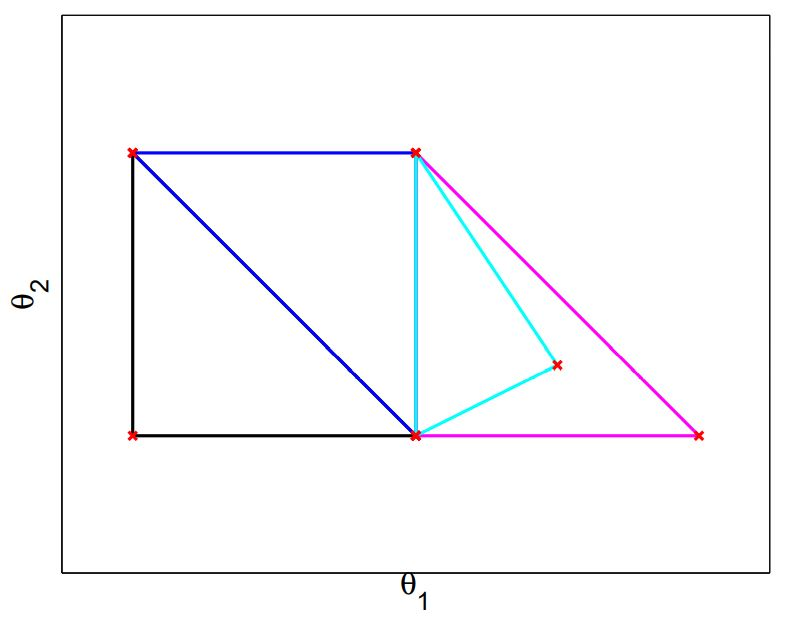
\includegraphics[width=\textwidth]{fig/18-4.jpg}
\end{columns}

\small
\textcolor{red}{Only the \underline{order}} of the function values matter:

$f(\hat{x})=1,f(\tilde{x})=1.0001$\,is the same as\,$f(\hat{x})=1,f(\tilde{x})=10000$.

$\textcolor{blue}{\rightarrow }$A very popular (in \underline{Numerical Recipes}), robust first choice

$\qquad$. . . with nontrivial convergence

\scriptsize
\flushright{Newer NM$\textcolor{blue}{\rightarrow}$\textcolor[RGB]{128,0,128}{ [Lagarias, Poonen, Wright; SIOPT 2012]}}
\end{frame}

%19
\begin{frame}{What Are We Missing?}
\begin{columns}
\column{0.8\textwidth}
These methods will (eventually) find a local solution

\scriptsize\flushright
Overview:$\textcolor{blue}{\rightarrow}$\textcolor[RGB]{128,0,128}{ [Kolda, Lewis, Torczon, SIREV 2003]}

\normalsize\flushleft
\colorbox[rgb]{0.5,0.6,0.7}{\textcolor{white}{Each evaluation of $f$ is expensive (\underline{valuable})}}

\column{0.1\textwidth}

\includegraphics[width=\textwidth]{fig/19.jpg}
\end{columns}

\vspace{0.2cm}
\begin{columns}
\column{0.45\textwidth}
N-M:
\begin{enumerate}\small
\item Only remembers the last $n+1$\,evaluations
\item Neglects the \underline{magnitudes} of the function values (order only)
\item Doesn’t take into account the special (LS) problem structure
\end{enumerate}

\column{0.45\textwidth}
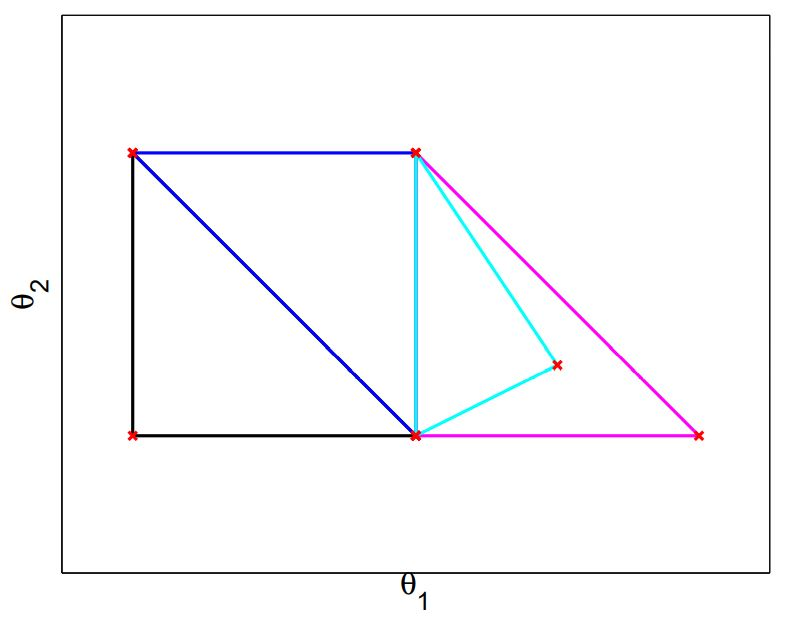
\includegraphics[width=\textwidth]{fig/18-4.jpg}
\end{columns}

\vspace{0.5cm}
$\textcolor{blue}{\rightarrow}$
This is the reason many direct search methods use a \underline{search} phase on top of the usual \underline{poll} phase
\end{frame}

%subsection
\subsection{Model-Based Methods}
%20-1
\begin{frame}{Making the Most of Little Information About Smooth $f$}
\begin{itemize}
\item $f$ is expensive $\Rightarrow$ can afford to make better use of points
\item Overhead of the optimization routine is minimal (\textcolor{blue}{negligible?}) relative to \textcolor{red}{cost of evaluating simulation}
\end{itemize}

\begin{columns}
\column{0.5\textwidth}
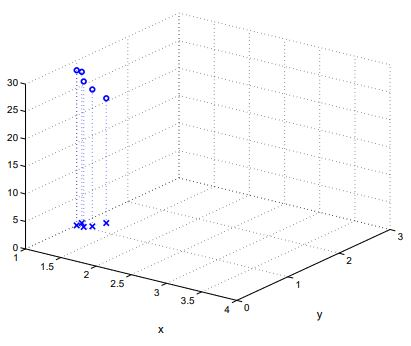
\includegraphics[width=\textwidth]{fig/20-1.jpg}

\column{0.5\textwidth}
\colorbox[rgb]{0.5,0.6,0.7}{\textcolor{white}{\underline{Bank} of data, $\{x^i,f(x^i)\}^k_{i=1}$:}}
\begin{itemize}
\item[\textcolor{blue}{=}] Points (\& function values) evaluated so far
\item[\textcolor{blue}{=}] Everything known about $f$
\end{itemize}

\colorbox[rgb]{0.5,0.6,0.7}{\textcolor{white}{Idea:}}
\begin{itemize}
\item Make use of growing \textcolor{blue}{Bank} as optimization progresses
\item Limit \textcolor{blue}{unnecessary} evaluations
\end{itemize}
\small\flushright
( \textcolor{blue}{geometry/approximation})
\end{columns}
\end{frame}

%20-2
\begin{frame}{Making the Most of Little Information About Smooth $f$}
\begin{itemize}
\item $f$ is expensive $\Rightarrow$ can afford to make better use of points
\item Overhead of the optimization routine is minimal (\textcolor{blue}{negligible?}) relative to \textcolor{red}{cost of evaluating simulation}
\end{itemize}

\begin{columns}
\column{0.5\textwidth}
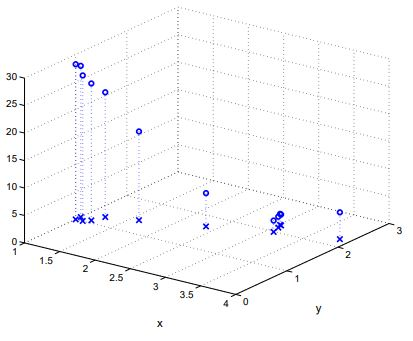
\includegraphics[width=\textwidth]{fig/20-2.jpg}

\column{0.5\textwidth}
\colorbox[rgb]{0.5,0.6,0.7}{\textcolor{white}{\underline{Bank} of data, $\{x^i,f(x^i)\}^k_{i=1}$:}}
\begin{itemize}
\item[\textcolor{blue}{=}] Points (\& function values) evaluated so far
\item[\textcolor{blue}{=}] Everything known about $f$
\end{itemize}

\colorbox[rgb]{0.5,0.6,0.7}{\textcolor{white}{Idea:}}
\begin{itemize}
\item Make use of growing \textcolor{blue}{Bank} as optimization progresses
\item Limit \textcolor{blue}{unnecessary} evaluations
\end{itemize}
\small\flushright
( \textcolor{blue}{geometry/approximation})
\end{columns}
\end{frame}

%21
\begin{frame}{Trust-Region Methods Use Models Instead of $f$}
To reduce the number of expensive $f$ evaluations
\begin{itemize}
\item[$\textcolor{blue}{\rightarrow}$] Replace difficult optimization problem $\textcolor{red}{\min f(x)}$ with a much simpler one $\textcolor{blue}{\min\{m(x) : x\in \mathcal{B}\}}$
\end{itemize}

\begin{columns}
\column{0.5\textwidth}
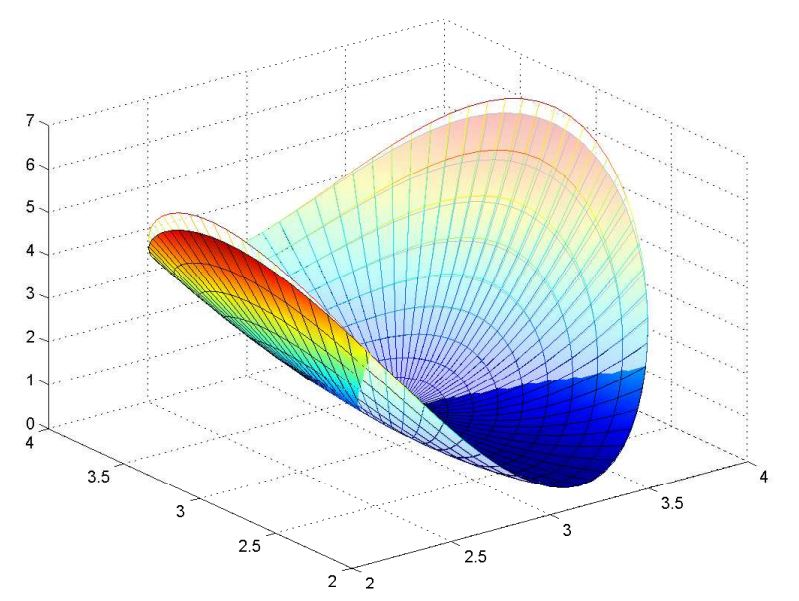
\includegraphics[width=\textwidth]{fig/21.jpg}

\column{0.5\textwidth}
\colorbox[rgb]{0.5,0.6,0.7}{\textcolor{white}{Classic NLP Technique:}}
\begin{itemize}
\item[$\textcolor{red}{f}$]  Original function: computationally expensive, no derivatives
\item[$\textcolor{blue}{m}$] Surrogate model: computationally attractive, analytic derivatives
\end{itemize}
\end{columns}
\end{frame}

%22-1
\begin{frame}{Basic Trust-Region Idea}
Use a model $\textcolor{blue}{m(x)}$ in place of the unwieldy $\textcolor{red}{f(x)}$

\begin{columns}
\column{0.5\textwidth}
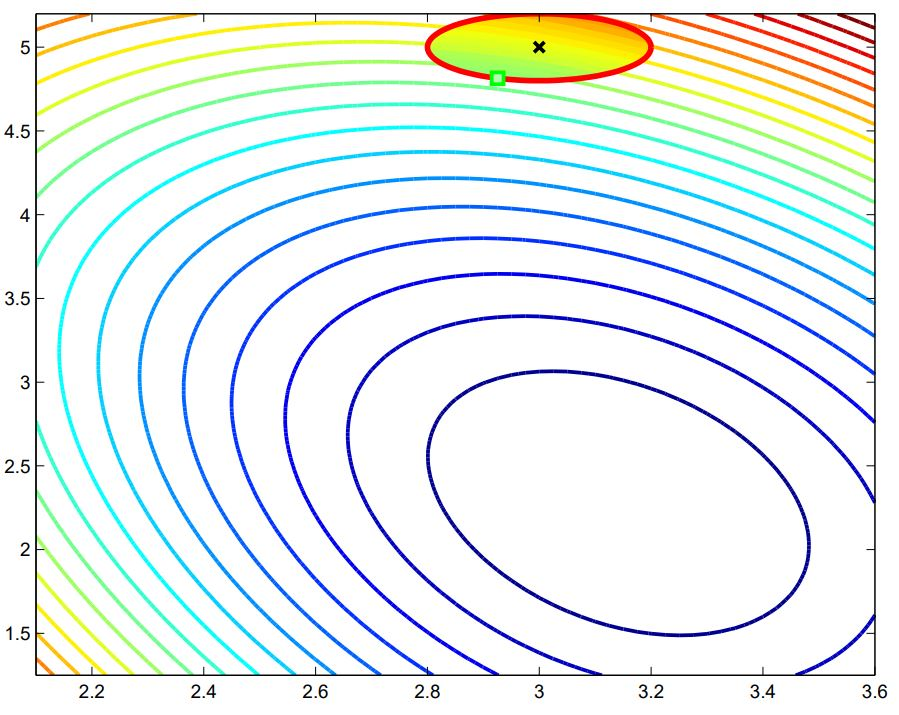
\includegraphics[width=\textwidth]{fig/22-1.jpg}

\column{0.5\textwidth}
\colorbox[rgb]{0.5,0.6,0.7}{\textcolor{white}{Optimize over }$\textcolor{blue}{m}$ \textcolor{white}{to avoidexpense }}

\colorbox[rgb]{0.5,0.6,0.7}{\textcolor{white}{of} $\textcolor{red}{f}$:}

\begin{itemize}
\item Trust $m$ to approximate $f$ within $ \mathcal{B}_k=\{x\in\mathbb{R}^n:||x-x^k||\le \Delta_k\}$
\item Obtain next point from $\min\{m(x^k+s):x^k+s\in \mathcal{B}_k\}$
\item Evaluate function and update $(x^k, \Delta_k)$\,based on how good the model's prediction was:
\begin{equation*}
\rho_k=\frac{f(x^k)-f(x^k+s^k)}{m(x^k)-m(x^k+s^k)}
\end{equation*}
\end{itemize}

\footnotesize\flushright{\textcolor[RGB]{128,0,128}{ [\underline{Conn, Gould, Toint}; SIAM, 2000]}}
\end{columns}
\end{frame}

%22-2
\begin{frame}{Basic Trust-Region Idea}
Use a model $\textcolor{blue}{m(x)}$ in place of the unwieldy $\textcolor{red}{f(x)}$

\begin{columns}
\column{0.5\textwidth}
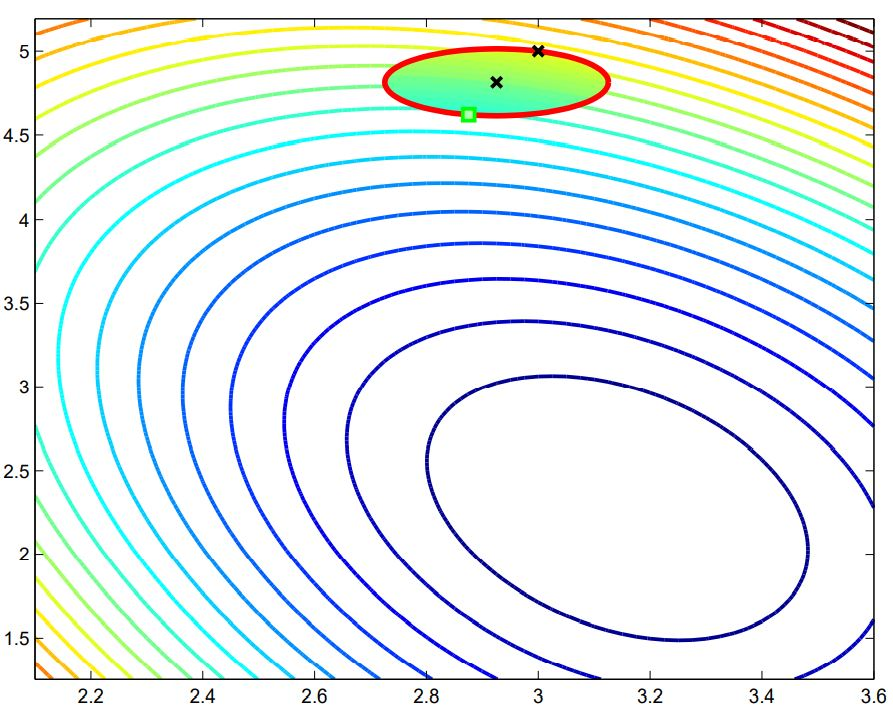
\includegraphics[width=\textwidth]{fig/22-2.jpg}

\column{0.5\textwidth}
\colorbox[rgb]{0.5,0.6,0.7}{\textcolor{white}{Optimize over }$\textcolor{blue}{m}$ \textcolor{white}{to avoidexpense }}

\colorbox[rgb]{0.5,0.6,0.7}{\textcolor{white}{of} $\textcolor{red}{f}$:}

\begin{itemize}
\item Trust $m$ to approximate $f$ within $ \mathcal{B}_k=\{x\in\mathbb{R}^n:||x-x^k||\le \Delta_k\}$
\item Obtain next point from $\min\{m(x^k+s):x^k+s\in \mathcal{B}_k\}$
\item Evaluate function and update $(x^k, \Delta_k)$\,based on how good the model's prediction was:
\begin{equation*}
\rho_k=\frac{f(x^k)-f(x^k+s^k)}{m(x^k)-m(x^k+s^k)}
\end{equation*}
\end{itemize}

\footnotesize\flushright{\textcolor[RGB]{128,0,128}{ [\underline{Conn, Gould, Toint}; SIAM, 2000]}}
\end{columns}
\end{frame}

%22-3
\begin{frame}{Basic Trust-Region Idea}
Use a model $\textcolor{blue}{m(x)}$ in place of the unwieldy $\textcolor{red}{f(x)}$

\begin{columns}
\column{0.5\textwidth}
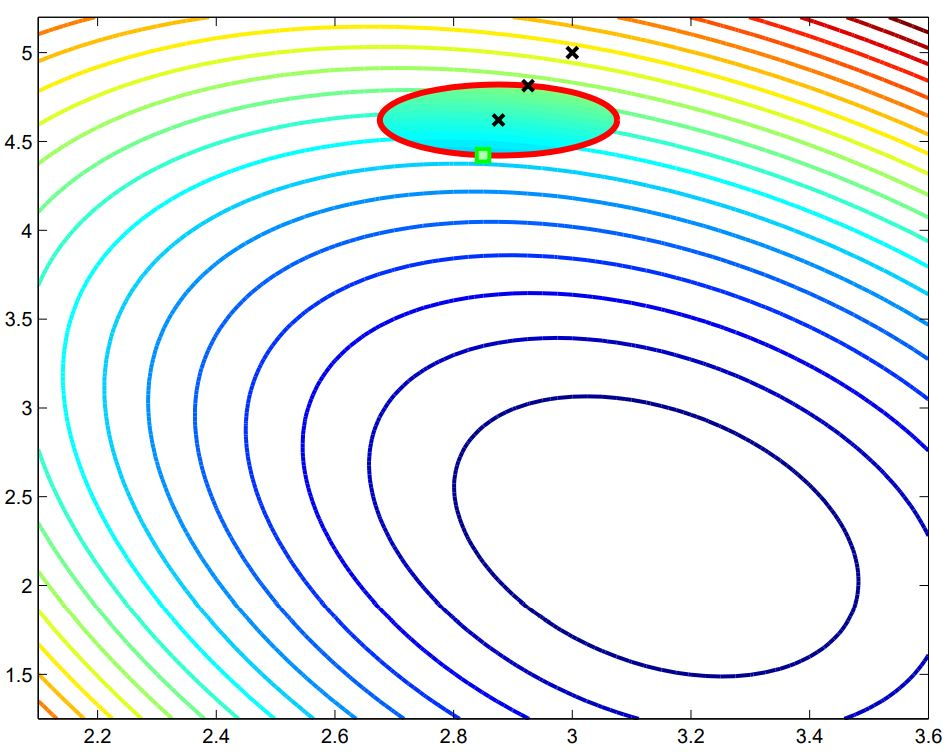
\includegraphics[width=\textwidth]{fig/22-3.jpg}

\column{0.5\textwidth}
\colorbox[rgb]{0.5,0.6,0.7}{\textcolor{white}{Optimize over }$\textcolor{blue}{m}$ \textcolor{white}{to avoidexpense }}

\colorbox[rgb]{0.5,0.6,0.7}{\textcolor{white}{of} $\textcolor{red}{f}$:}

\begin{itemize}
\item Trust $m$ to approximate $f$ within $ \mathcal{B}_k=\{x\in\mathbb{R}^n:||x-x^k||\le \Delta_k\}$
\item Obtain next point from $\min\{m(x^k+s):x^k+s\in  \mathcal{B}_k\}$
\item Evaluate function and update $(x^k, \Delta_k)$\,based on how good the model's prediction was:
\begin{equation*}
\rho_k=\frac{f(x^k)-f(x^k+s^k)}{m(x^k)-m(x^k+s^k)}
\end{equation*}
\end{itemize}

\footnotesize\flushright{\textcolor[RGB]{128,0,128}{ [\underline{Conn, Gould, Toint}; SIAM, 2000]}}
\end{columns}
\end{frame}

%22-4
\begin{frame}{Basic Trust-Region Idea}
Use a model $\textcolor{blue}{m(x)}$ in place of the unwieldy $\textcolor{red}{f(x)}$

\begin{columns}
\column{0.5\textwidth}
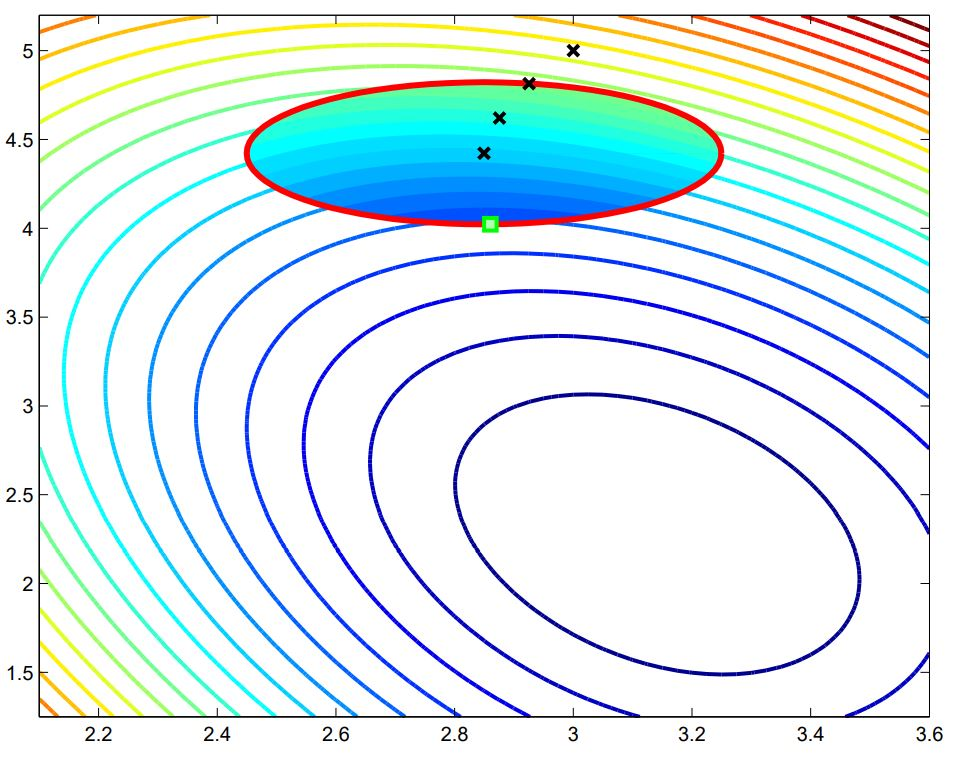
\includegraphics[width=\textwidth]{fig/22-4.jpg}

\column{0.5\textwidth}
\colorbox[rgb]{0.5,0.6,0.7}{\textcolor{white}{Optimize over }$\textcolor{blue}{m}$ \textcolor{white}{to avoidexpense }}

\colorbox[rgb]{0.5,0.6,0.7}{\textcolor{white}{of} $\textcolor{red}{f}$:}

\begin{itemize}
\item Trust $m$ to approximate $f$ within $ \mathcal{B}_k=\{x\in\mathbb{R}^n:||x-x^k||\le \Delta_k\}$
\item Obtain next point from $\min\{m(x^k+s):x^k+s\in  \mathcal{B}_k\}$
\item Evaluate function and update $(x^k, \Delta_k)$\,based on how good the model's prediction was:
\begin{equation*}
\rho_k=\frac{f(x^k)-f(x^k+s^k)}{m(x^k)-m(x^k+s^k)}
\end{equation*}
\end{itemize}

\footnotesize\flushright{\textcolor[RGB]{128,0,128}{ [\underline{Conn, Gould, Toint}; SIAM, 2000]}}
\end{columns}
\end{frame}

%22-5
\begin{frame}{Basic Trust-Region Idea}
Use a model $\textcolor{blue}{m(x)}$ in place of the unwieldy $\textcolor{red}{f(x)}$

\begin{columns}
\column{0.5\textwidth}
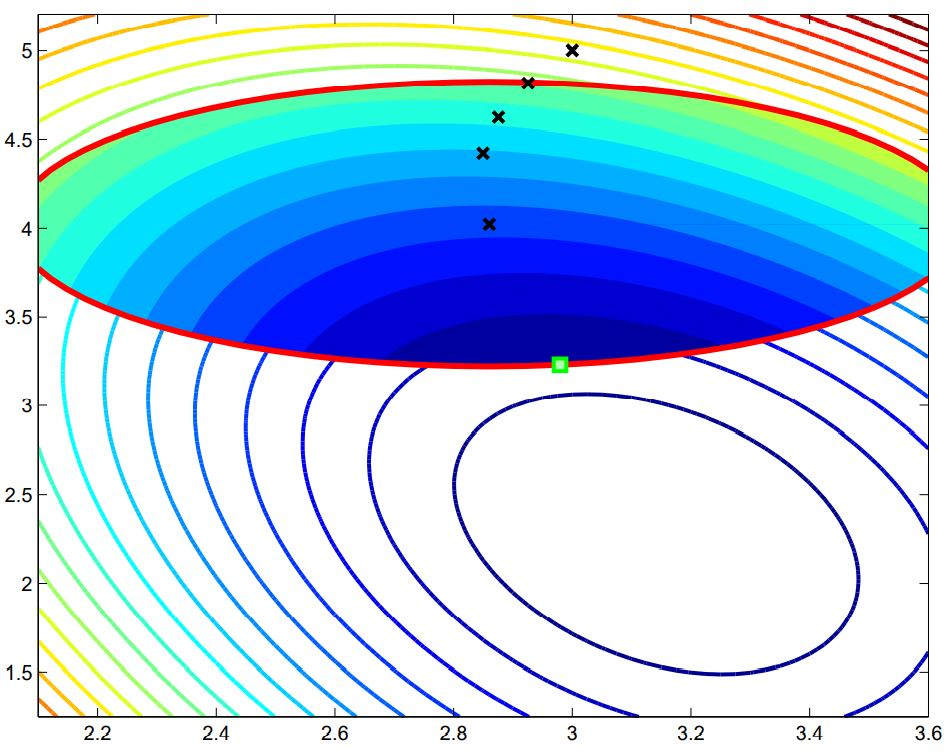
\includegraphics[width=\textwidth]{fig/22-5.jpg}

\column{0.5\textwidth}
\colorbox[rgb]{0.5,0.6,0.7}{\textcolor{white}{Optimize over }$\textcolor{blue}{m}$ \textcolor{white}{to avoidexpense }}

\colorbox[rgb]{0.5,0.6,0.7}{\textcolor{white}{of} $\textcolor{red}{f}$:}

\begin{itemize}
\item Trust $m$ to approximate $f$ within $ \mathcal{B}_k=\{x\in\mathbb{R}^n:||x-x^k||\le \Delta_k\}$
\item Obtain next point from $\min\{m(x^k+s):x^k+s\in  \mathcal{B}_k\}$
\item Evaluate function and update $(x^k, \Delta_k)$\,based on how good the model's prediction was:
\begin{equation*}
\rho_k=\frac{f(x^k)-f(x^k+s^k)}{m(x^k)-m(x^k+s^k)}
\end{equation*}
\end{itemize}

\footnotesize\flushright{\textcolor[RGB]{128,0,128}{ [\underline{Conn, Gould, Toint}; SIAM, 2000]}}
\end{columns}
\end{frame}

%22-6
\begin{frame}{Basic Trust-Region Idea}
Use a model $\textcolor{blue}{m(x)}$ in place of the unwieldy $\textcolor{red}{f(x)}$

\begin{columns}
\column{0.5\textwidth}
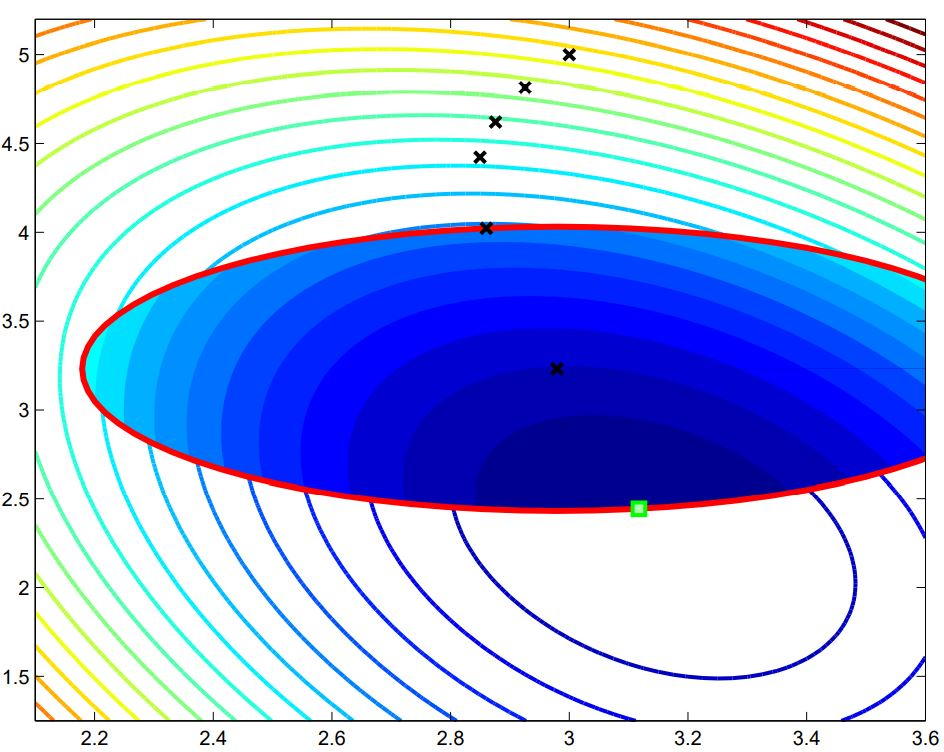
\includegraphics[width=\textwidth]{fig/22-6.jpg}

\column{0.5\textwidth}
\colorbox[rgb]{0.5,0.6,0.7}{\textcolor{white}{Optimize over }$\textcolor{blue}{m}$ \textcolor{white}{to avoidexpense }}

\colorbox[rgb]{0.5,0.6,0.7}{\textcolor{white}{of} $\textcolor{red}{f}$:}

\begin{itemize}
\item Trust $m$ to approximate $f$ within $ \mathcal{B}_k=\{x\in\mathbb{R}^n:||x-x^k||\le \Delta_k\}$
\item Obtain next point from $\min\{m(x^k+s):x^k+s\in  \mathcal{B}_k\}$
\item Evaluate function and update $(x^k, \Delta_k)$\,based on how good the model's prediction was:
\begin{equation*}
\rho_k=\frac{f(x^k)-f(x^k+s^k)}{m(x^k)-m(x^k+s^k)}
\end{equation*}
\end{itemize}

\footnotesize\flushright{\textcolor[RGB]{128,0,128}{ [\underline{Conn, Gould, Toint}; SIAM, 2000]}}
\end{columns}
\end{frame}

%22-7
\begin{frame}{Basic Trust-Region Idea}
Use a model $\textcolor{blue}{m(x)}$ in place of the unwieldy $\textcolor{red}{f(x)}$

\begin{columns}
\column{0.5\textwidth}
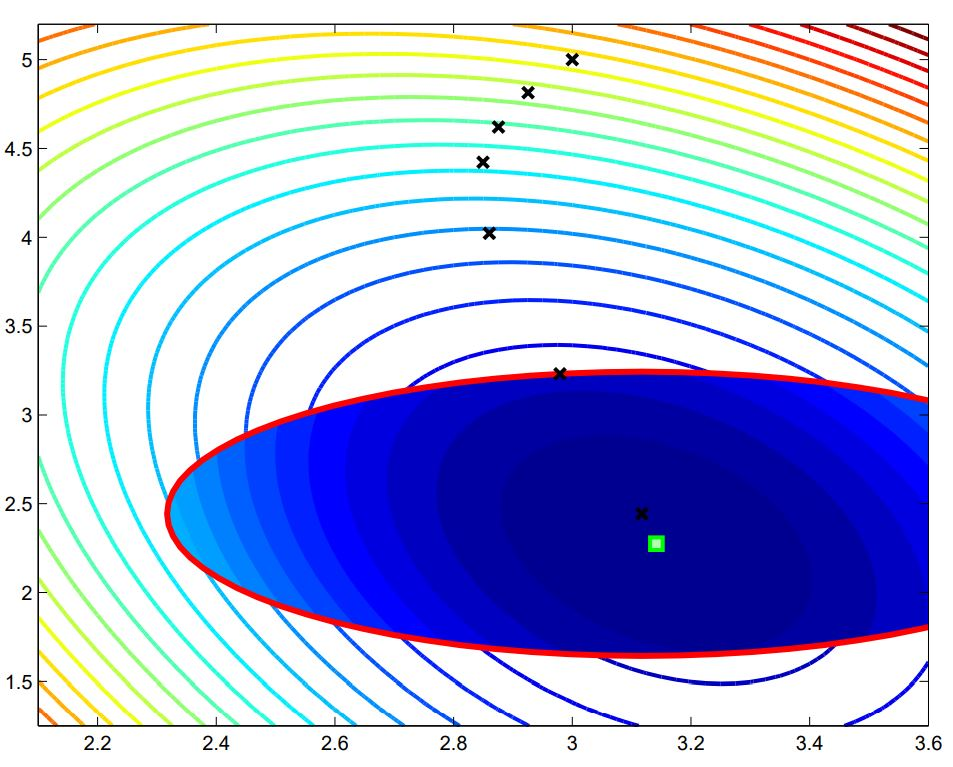
\includegraphics[width=\textwidth]{fig/22-7.jpg}

\column{0.5\textwidth}
\colorbox[rgb]{0.5,0.6,0.7}{\textcolor{white}{Optimize over }$\textcolor{blue}{m}$ \textcolor{white}{to avoidexpense }}

\colorbox[rgb]{0.5,0.6,0.7}{\textcolor{white}{of} $\textcolor{red}{f}$:}

\begin{itemize}
\item Trust $m$ to approximate $f$ within $ \mathcal{B}_k=\{x\in\mathbb{R}^n:||x-x^k||\le \Delta_k\}$
\item Obtain next point from $\min\{m(x^k+s):x^k+s\in  \mathcal{B}_k\}$
\item Evaluate function and update $(x^k, \Delta_k)$\,based on how good the model's prediction was:
\begin{equation*}
\rho_k=\frac{f(x^k)-f(x^k+s^k)}{m(x^k)-m(x^k+s^k)}
\end{equation*}
\end{itemize}

\footnotesize\flushright{\textcolor[RGB]{128,0,128}{ [\underline{Conn, Gould, Toint}; SIAM, 2000]}}
\end{columns}
\end{frame}

%23-1
\begin{frame}{Where Does the Model Come From?}
\colorbox[rgb]{0.5,0.6,0.7}{\textcolor{white}{When derivatives are available:}}

\begin{tabular}{rl}
\textcolor{blue}{Taylor-based} & model\,$m(x^k+s)=c+(g^k)^Ts+\frac{1}{2}s^TH^ks$\\
& $\quad g^k=\nabla_xf(x^k)$\\
& $\quad H^k\approx\nabla_{x,x}^2f(x^k)$
%& \begin{itemize}
%\item $g^k=\nabla_xf(x^k)$
%\item $H^k\approx\nabla_{x,x}^2f(x^k)$
%\end{itemize}
\end{tabular}

\vspace{2.2cm}
\end{frame}

%23-2
\begin{frame}{Where Does the Model Come From?}
\colorbox[rgb]{0.5,0.6,0.7}{\textcolor{white}{When derivatives are available:}}

\begin{tabular}{rl}
\textcolor{blue}{Taylor-based} & model\,$m(x^k+s)=c+(g^k)^Ts+\frac{1}{2}s^TH^ks$\\
& $\quad g^k=\nabla_xf(x^k)$\\
& $\quad H^k\approx\nabla_{x,x}^2f(x^k)$
%& \begin{itemize}
%\item $g^k=\nabla_xf(x^k)$
%\item $H^k\approx\nabla_{x,x}^2f(x^k)$
%\end{itemize}
\end{tabular}

\colorbox[rgb]{0.5,0.6,0.7}{\textcolor{white}{Without derivatives}}
\begin{itemize}
\item Interpolation-based models
\item Regression-based models
\item Stochastic/randomized models
\end{itemize}
\end{frame}

%24
\begin{frame}{Interpolation-Based Quadratic Models}
\begin{columns}
\column{0.5\textwidth}
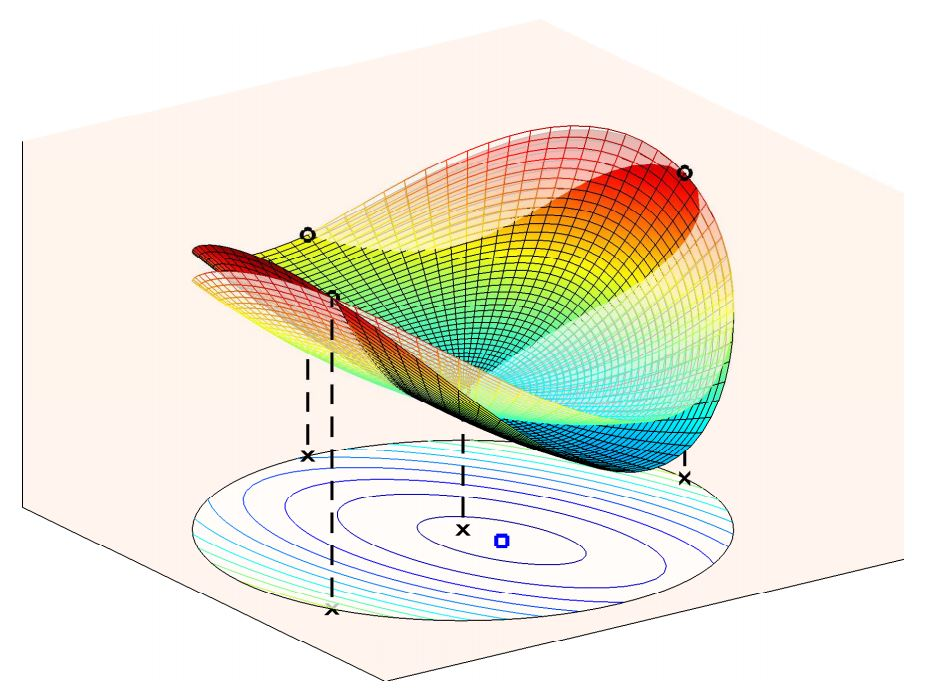
\includegraphics[width=\textwidth]{fig/24.jpg}

\begin{center}
An interpolating quadratic in $\mathbb{R}^2$
\end{center}

\column{0.5\textwidth}
\colorbox[rgb]{0.5,0.6,0.7}{\textcolor{white}{$m(x^k+s)=c+g^Ts+\frac{1}{2}s^THs$:}}

Get the model parameters $c,g,H = H^T$ by demanding interpolation:
\begin{equation*}
m(x^k+y^i)=f(x^k+y^i)
\end{equation*}
for all $y^i\in\mathcal{Y}=$ interpolation set

\colorbox[rgb]{0.5,0.6,0.7}{\textcolor{white}{Main difficulty is $\mathcal{Y}$:}}

\begin{itemize}
\item Use prior function evaluations,
\item $m$ well-defined and approximates $f$ locally.
\end{itemize}
\end{columns}
\end{frame}

%25-1
\begin{frame}{Interpolation-Based Trust-Region Methods}
\begin{columns}
\column{0.6\textwidth}
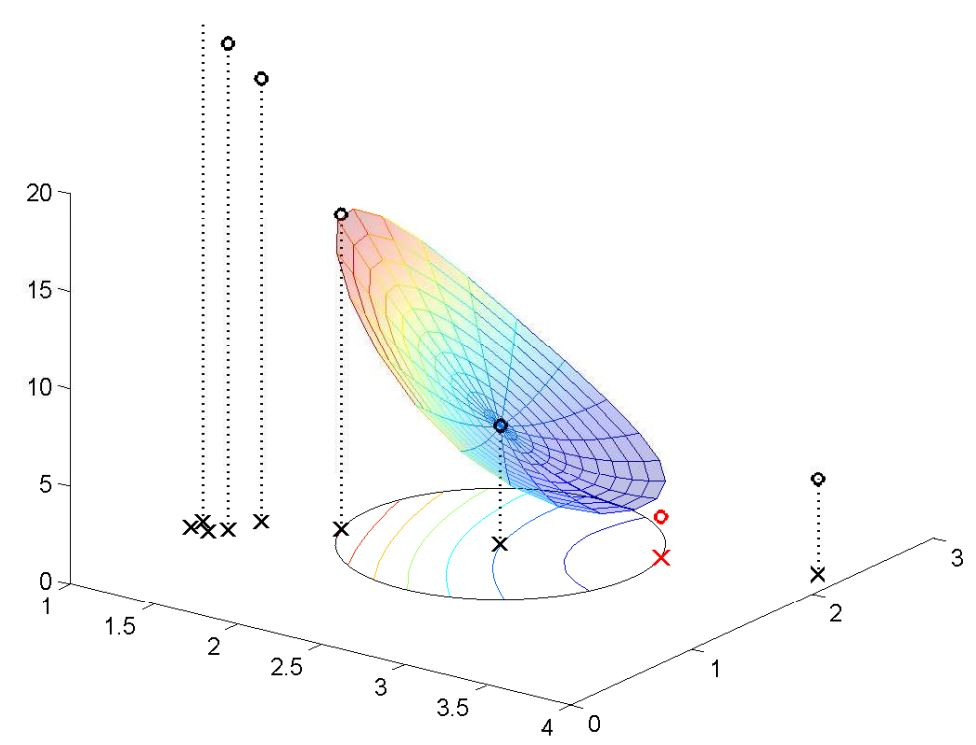
\includegraphics[width=\textwidth]{fig/25-1.jpg}

\column{0.4\textwidth}
\colorbox[rgb]{0.5,0.6,0.7}{\textcolor{white}{Iteration $k$:}}
\begin{itemize}\small
\item  Build a model $m_k$ interpolating $f$ on $\mathcal{Y}$
\item Trust $m_k$ within region $\mathcal{B}_k$
\item Minimize $m_k$ within $\mathcal{B}_k$ to obtain next point for evaluation
\item Do expensive evaluation
\item Update $m_k$ and $\mathcal{B}_k$ based on how good model prediction was
\end{itemize}
\end{columns}
\end{frame}

%25-2
\begin{frame}{Interpolation-Based Trust-Region Methods}
\begin{columns}
\column{0.6\textwidth}
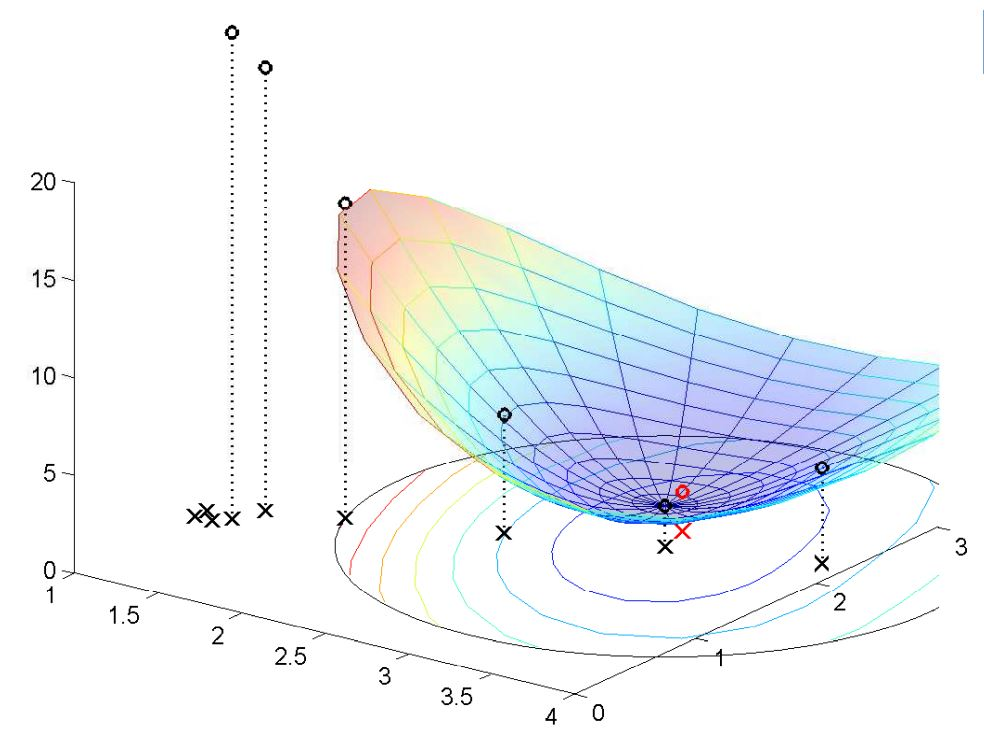
\includegraphics[width=\textwidth]{fig/25-2.jpg}

\column{0.4\textwidth}
\colorbox[rgb]{0.5,0.6,0.7}{\textcolor{white}{Iteration $k$:}}
\begin{itemize}\small
\item  Build a model $m_k$ interpolating $f$ on $\mathcal{Y}$
\item Trust $m_k$ within region $\mathcal{B}_k$
\item Minimize $m_k$ within $\mathcal{B}_k$ to obtain next point for evaluation
\item Do expensive evaluation
\item Update $m_k$ and $\mathcal{B}_k$ based on how good model prediction was
\end{itemize}
\end{columns}
\end{frame}

%25-3
\begin{frame}{Interpolation-Based Trust-Region Methods}
\begin{columns}
\column{0.6\textwidth}
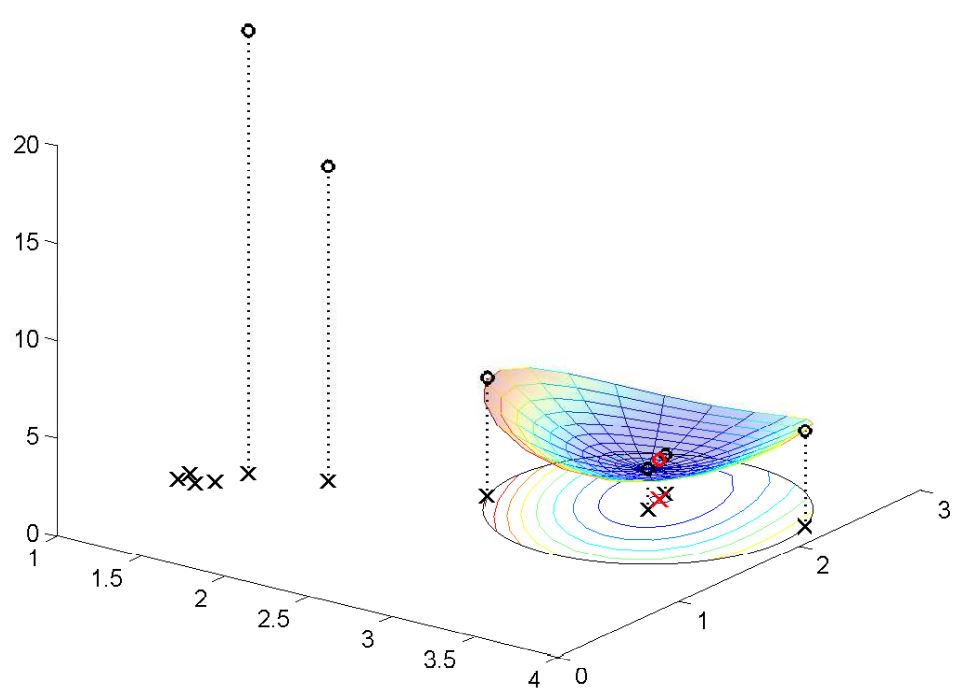
\includegraphics[width=\textwidth]{fig/25-3.jpg}

\column{0.4\textwidth}
\colorbox[rgb]{0.5,0.6,0.7}{\textcolor{white}{Iteration $k$:}}
\begin{itemize}\small
\item  Build a model $m_k$ interpolating $f$ on $\mathcal{Y}$
\item Trust $m_k$ within region $\mathcal{B}_k$
\item Minimize $m_k$ within $\mathcal{B}_k$ to obtain next point for evaluation
\item Do expensive evaluation
\item Update $m_k$ and $\mathcal{B}_k$ based on how good model prediction was
\end{itemize}
\end{columns}
\end{frame}

%25-4
\begin{frame}{Interpolation-Based Trust-Region Methods}
\begin{columns}
\column{0.6\textwidth}
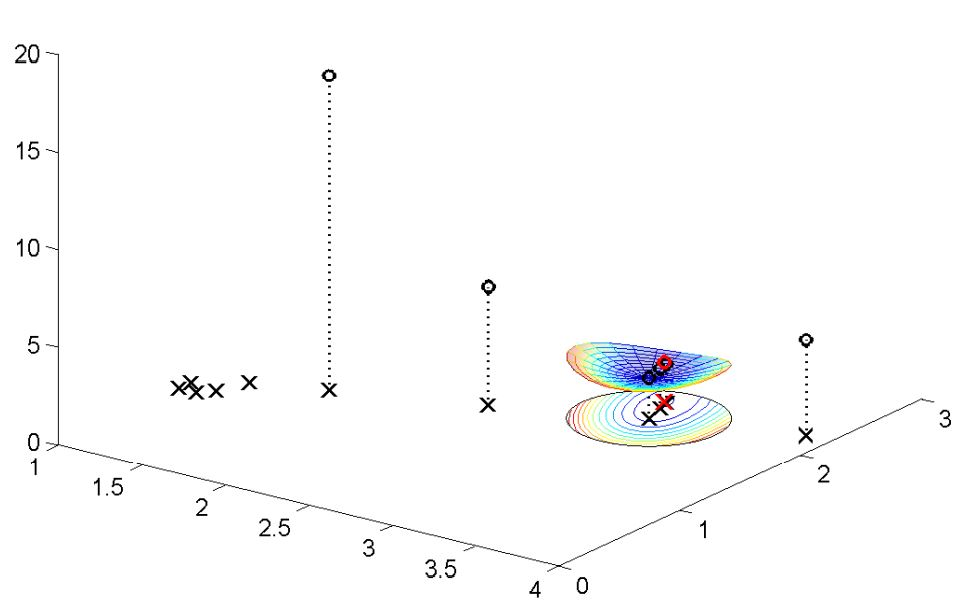
\includegraphics[width=\textwidth]{fig/25-4.jpg}

\column{0.4\textwidth}
\colorbox[rgb]{0.5,0.6,0.7}{\textcolor{white}{Iteration $k$:}}
\begin{itemize}\small
\item  Build a model $m_k$ interpolating $f$ on $\mathcal{Y}$
\item Trust $m_k$ within region $\mathcal{B}_k$
\item Minimize $m_k$ within $\mathcal{B}_k$ to obtain next point for evaluation
\item Do expensive evaluation
\item Update $m_k$ and $\mathcal{B}_k$ based on how good model prediction was
\end{itemize}
\end{columns}
\end{frame}

%26-1
\begin{frame}{Quick Diversion: Polynomial Bases}
\begin{itemize}
\item Let $\phi$ denote a basis for some space of polynomials of $n$ variables
	\begin{itemize}
	\item Linear:
\begin{equation*}
\phi(x)=[1,x_1,\cdots,x_n]
\end{equation*}
	\end{itemize}
\end{itemize}
\vspace{5.5cm}
\end{frame}

%26-2
\begin{frame}{Quick Diversion: Polynomial Bases}
\begin{itemize}
\item Let $\phi$ denote a basis for some space of polynomials of $n$ variables
	\begin{itemize}
	\item Linear:
\begin{equation*}
\phi(x)=[1,x_1,\cdots,x_n]
\end{equation*}
	\item Full quadratics:
\begin{equation*}
\phi(x)=[1,x_1,\cdots,x_n,x_1^2,\cdots,x_n^2,x_1x_2,\cdots,x_{n-1}x_n]
\end{equation*}
	\end{itemize}
\end{itemize}
\vspace{4cm}
\end{frame}

%26-3
\begin{frame}{Quick Diversion: Polynomial Bases}
\begin{itemize}
\item Let $\phi$ denote a basis for some space of polynomials of $n$ variables
	\begin{itemize}
	\item Linear:
\begin{equation*}
\phi(x)=[1,x_1,\cdots,x_n]
\end{equation*}
	\item Full quadratics:
\begin{equation*}
\phi(x)=[1,x_1,\cdots,x_n,x_1^2,\cdots,x_n^2,x_1x_2,\cdots,x_{n-1}x_n]
\end{equation*}
	\end{itemize}
\item Given a collection of $p=|\mathcal{Y}|$ points $\mathcal{Y}=\{y^1,...y^p\}$:

\begin{equation*}
\Phi(\mathcal{Y})=
\begin{bmatrix}
1 & y_1^1 & \cdots & y_n^1 &(y_1^1)^2 & \cdots & (y_n^1)^2 & y_1^1y_2^1 & \cdots & y_{n-1}^1y_n^1\\ 
\vdots&&&&&&&&&\vdots \\
1 & y_1^p & \cdots & y_n^p & (y_1^p)^2 & \cdots & (y_n^p)^2 & y_1^py_2^p & \cdots & y_{n-1}^py_n^p
\end{bmatrix}
\end{equation*}

This is a matrix of size $p\times\frac{(n+1)(n+2)}{2}$
\end{itemize}
\end{frame}

%27
\begin{frame}{Building Models Without Derivatives}
\small
Given data $(\mathcal{Y}^k,f(\mathcal{Y}^k))$ and basis $\Phi$, “solve”
\begin{equation*}
\Phi(\mathcal{Y}^k)z=[\Phi_c\quad\Phi_g\quad\Phi_H]
\begin{bmatrix}
z_c\\
z_g\\
z_H
\end{bmatrix}
=\underline{\textup{f}}=f(\mathcal{Y}^k)
\end{equation*}

\begin{columns}
\column{0.5\textwidth}
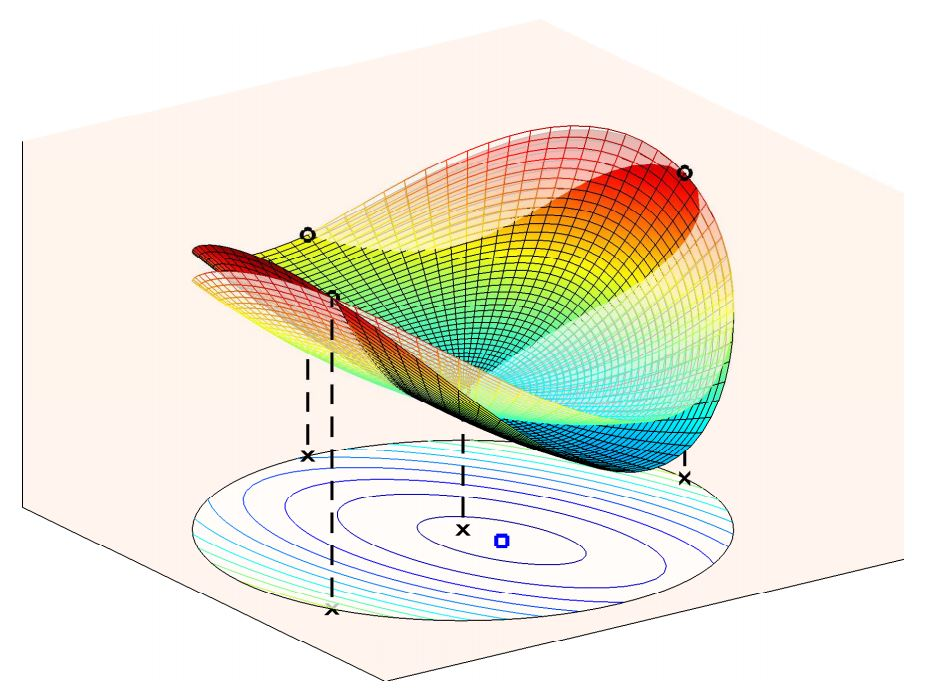
\includegraphics[width=\textwidth]{fig/24.jpg}

\begin{center}
$n=2,|\mathcal{Y}^k|=4$
\end{center}

\column{0.5\textwidth}
\colorbox[rgb]{0.5,0.6,0.7}{\textcolor{white}{Full quadratics, $|\mathcal{Y}^k|=\frac{(n+1)(n+2)}{2}$}}
\begin{itemize}\footnotesize
\item Geometric conditions on points in $\mathcal{Y}^k$
\end{itemize}

\colorbox[rgb]{0.5,0.6,0.7}{\textcolor{white}{Undetermined interpolation, }}
\colorbox[rgb]{0.5,0.6,0.7}{\textcolor{white}{$|\mathcal{Y}^k|<\frac{(n+1)(n+2)}{2}$}}
\begin{itemize}\footnotesize
\item Use \textcolor{blue}{(Powell)} Hessian updates

\begin{tabular}{rl}
$\textup{min}_{g^k, H^k}$ & $||H^k-H^{k-1}||^2_F$\\
s.t. & $q_k=\underline{\textup{f}}$ on $\mathcal{Y}^k$
\end{tabular}

\end{itemize}

\colorbox[rgb]{0.5,0.6,0.7}{\textcolor{white}{Regression, $|\mathcal{Y}^k|>\frac{(n+1)(n+2)}{2}$}}
\begin{itemize}\footnotesize
\item Solve $\textup{min}_z||\Phi_z-\underline{\textup{f}}||$
\end{itemize}
\end{columns}
\end{frame}

%28
\begin{frame}{Multivariate (Scattered Data) Interpolation is a Different Kind of Animal}
\begin{equation*}
m(x^k+y^i)=f(x^k+y^i)\quad\forall y^i\in\mathcal{Y}
\end{equation*}

\begin{itemize}
\item[\textcolor{blue}{n=1}] Given $p$ distinct points, can find a unique degree $p-1$ polynomial $m$
\item[\textcolor{blue}{n>1}] \textcolor{red}{Not true!} (see \textcolor{blue}{Mairhuber-Curtis Theorem})
\end{itemize}

\begin{columns}
\column{0.47\textwidth}
\colorbox[rgb]{0.5,0.6,0.7}{\textcolor{white}{For quadratic models in $\mathbb{R}^n$:}}
\begin{itemize}\small
\item $\frac{(n+1)(n+2)}{2}$ coefficients
\item Unique interpolant may not exist, even when $\mathcal{Y}=\frac{(n+1)(n+2)}{2}$
\item Locations of the points in $\mathcal{Y}$ must satisfy additional \textcolor{blue}{geometric} conditions 
\underline{(has nothing to do with $f$ values)}
\end{itemize}

\column{0.53\textwidth}
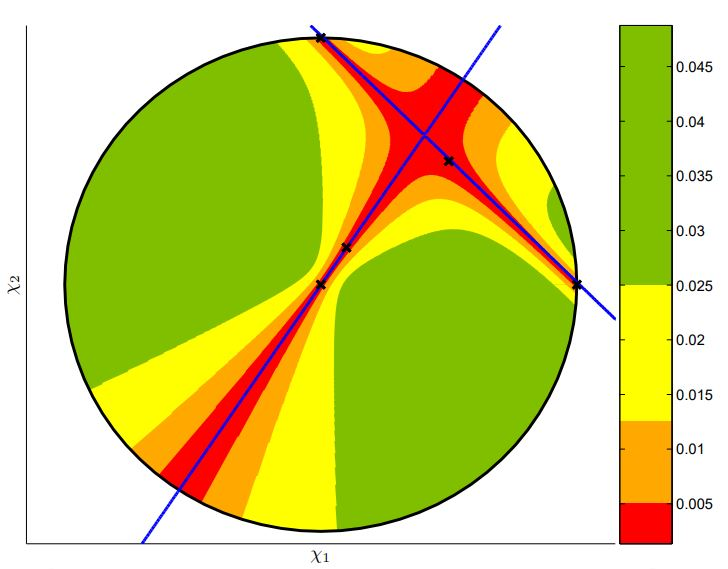
\includegraphics[width=\textwidth]{fig/28.jpg}
\scriptsize\flushright{\textcolor{blue}{$\rightarrow$}\textcolor[RGB]{128,0,128}{[\underline{ Wendland}; Cambridge University Press, 2010]}}
\end{columns}
\end{frame}

%29-1
\begin{frame}{Notions of Nonlinear Model Quality}
\colorbox[rgb]{0.5,0.6,0.7}{\textcolor{white}{“Taylor-like” Error Bounds}}
\begin{enumerate}
\item Assuming underlying $f$ is sufficiently smooth

\textcolor{blue}{=} derivatives of $f$ exist but are unavailable

\item A model $m_k$ is locally \textcolor{blue}{fully linear} if:

For all $x\in\mathcal{B}_k=\{x\in\Omega:||x-x^k||\le\Delta_k\}$
	\begin{itemize}
	\item $|m_k(x)-f(x)|\le\kappa_1\Delta^2_k$
	\item $||\nabla m_k(x)-\nabla f(x)||\le\kappa_2\Delta_k$
	\end{itemize}
for constants $\kappa_i$ independent of $x$ and $\Delta_k$.
\end{enumerate}

\scriptsize\flushright{\textcolor{blue}{$\rightarrow$}\textcolor[RGB]{128,0,128}{[\underline{ Conn, Scheinberg, Vicente}; SIAM 2009]}}
\end{frame}

%29-2
\begin{frame}{Notions of Nonlinear Model Quality}
\colorbox[rgb]{0.5,0.6,0.7}{\textcolor{white}{“Taylor-like” Error Bounds}}
\begin{enumerate}
\item Assuming underlying $f$ is sufficiently smooth

\item A model $m_k$ is locally \textcolor{blue}{fully linear} if:

For all $x\in\mathcal{B}_k=\{x\in\Omega:||x-x^k||\le\Delta_k\}$
	\begin{itemize}
	\item $|m_k(x)-f(x)|\le\kappa_1\Delta^3_k$
	\item $||\nabla m_k(x)-\nabla f(x)||\le\kappa_2\Delta^2_k$
	\item $||\nabla^2 m_k(x)-\nabla^2 f(x)||\le\kappa_3\Delta_k$
	\end{itemize}
for constants $\kappa_i$ independent of $x$ and $\Delta_k$.
\end{enumerate}

\scriptsize\flushright{\textcolor{blue}{$\rightarrow$}\textcolor[RGB]{128,0,128}{[\underline{ Conn, Scheinberg, Vicente}; SIAM 2009]}}
\end{frame}

%30
\begin{frame}{Ingredients for Convergence to Stationary Points}
\footnotesize
\colorbox[rgb]{0.5,0.6,0.7}{\textcolor{white}{$\textup{lim}_{k\rightarrow\infty}\nabla f(x^k)=0$  provided:}}
\begin{enumerate}[0]
\item $f$ is \textcolor{red}{sufficiently smooth} and regular (e.g., bounded level sets)
\end{enumerate}
\begin{enumerate}[1]
\item Control $\mathcal{B}_k$ based on model quality
\end{enumerate}
\begin{enumerate}[2]
\item  (Occasional) approximation within $\mathcal{B}_k$

Our quadratics satisfy
	\begin{itemize}
	\item $|q_k(x)-f(x)|\le\kappa_1(\gamma_f+||H^k||)\Delta_k^2,\quad x\in\mathcal{B}_k$
	\item $||g^k+H^k(x-x^k)-\nabla f(x)||\le\kappa_2(\gamma_f+||H^k||)\Delta_k,\quad x\in\mathcal{B}_k$
	\end{itemize}
\end{enumerate}
\begin{enumerate}[3]
\item Sufficient decrease
\end{enumerate}

\rule{\textwidth}{1pt}

\begin{columns}
\tiny
\column{0.35\textwidth}
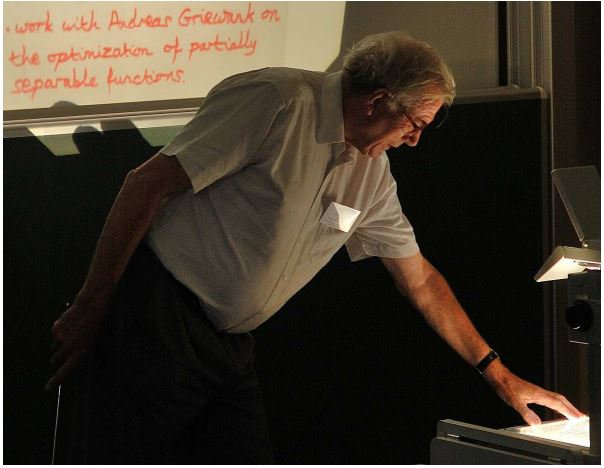
\includegraphics[width=\textwidth]{fig/30.jpg}
\begin{center}
Michael J.D. Powell, 1936-2015
\end{center}

\column{0.6\textwidth}
\tiny\flushright
Survey \textcolor{blue}{$\rightarrow$}\textcolor[RGB]{128,0,128}{[\underline{ Conn, Scheinberg, Vicente}; SIAM 2009]}

Methods \textcolor{blue}{$\rightarrow$}\textcolor[RGB]{128,0,128}{[Powell: COBYLA, UOBYQA, NEWUOA, BOBYQA, LINCOA],}

. . .

Line search methods also work \textcolor{blue}{$\rightarrow$}\textcolor[RGB]{128,0,128}{[Kelley et al; IFFCO]}

RBF models also work \textcolor{blue}{$\rightarrow$}\textcolor[RGB]{128,0,128}{[W. \& Shoemaker; SIREV 2013]}

Probabilistic models\textcolor{blue}{$\rightarrow$}\textcolor[RGB]{128,0,128}{[Bandeira, Scheinberg, Vicente; SIOPT 2014]}
\end{columns}
\end{frame}

%31
\begin{frame}{Greed. Alone. Can. Hurt.}
Model-improvement may be needed when:
\begin{itemize}
\item Nearby points line up
\item May not have enough points to ensure model quality in all directions
\end{itemize}

\begin{center}
\includegraphics[width=0.5\textwidth]{fig/31.jpg}
\end{center}

\textcolor{red}{$\rightarrow$} May need $n$ \textcolor{red}{additional evaluations}
\end{frame}

%32
\begin{frame}{Constraints and Model Quality}
\begin{center}
\textcolor{red}{Constraints complicate matters}

\textcolor{red}{. . . if one does not allow evaluation of infeasible points}

\includegraphics[width=0.85\textwidth]{fig/32.jpg}
\end{center}

\textcolor{red}{$\rightarrow$} May need directions normal to nearby constraints
\end{frame}

%33-1
\begin{frame}{Performance Comparisons on Test Functions}
\begin{columns}
\column{0.6\textwidth}
\includegraphics[width=\textwidth]{fig/33-1.jpg}

\begin{center}
Smooth problems
\end{center}

\column{0.35\textwidth}
\begin{itemize}\footnotesize
\item When evaluations are sequential, \textcolor{blue}{model-based methods} (\textcolor{red}{NEWUOA}) regularly outperform direct search methods without a search phase (\textcolor{blue}{nmsmax}, \textbf{appsrand})
\end{itemize}
\scriptsize
\textcolor{blue}{$\rightarrow$}\textcolor[RGB]{128,0,128}{[Mor$\acute{\textup{e}}$ \& W., SIOPT 2009]}
\end{columns}
\end{frame}

%33-2
\begin{frame}{Performance Comparisons on Test Functions}
\begin{columns}
\column{0.6\textwidth}
\includegraphics[width=\textwidth]{fig/33-2.jpg}

\begin{center}
Noisy problems
\end{center}

\column{0.35\textwidth}
\begin{itemize}\footnotesize
\item When evaluations are sequential, \textcolor{blue}{model-based methods} (\textcolor{red}{NEWUOA}) regularly outperform direct search methods without a search phase (\textcolor{blue}{nmsmax}, \textbf{appsrand})
\end{itemize}
\scriptsize
\textcolor{blue}{$\rightarrow$}\textcolor[RGB]{128,0,128}{[Mor$\acute{\textup{e}}$ \& W., SIOPT 2009]}
\end{columns}
\end{frame}

%34-1
\begin{frame}{Many Practical Details In Implementations}
\begin{itemize}
\item Choice of interpolation points $\mathcal{Y}^k$
\item Updating of trust region $\mathcal{B}_k$
\item Improvement of models
\end{itemize}

\vspace{5.5cm}
\end{frame}

%34-2
\begin{frame}{Many Practical Details In Implementations}
\begin{itemize}
\item Choice of interpolation points $\mathcal{Y}^k$
\item Updating of trust region $\mathcal{B}_k$
\item Improvement of models
\end{itemize}

\ttfamily
\textcolor{red}{BOBYQA [Powell]},\textcolor[RGB]{0,130,80}{DFO [Scheinberg]},\textcolor[RGB]{128,0,128}{POUNDer [W.]}
\sffamily

\begin{table}[]\small
\begin{tabular}{rl}
Initialization   & \textcolor{red}{$p=|\mathcal{Y}^k|$ structured evaluations} \\
&\textcolor[RGB]{0,130,80}{Based on input, $\approx 2n+1$}\\
&\textcolor[RGB]{128,0,128}{Based on input, no more than n+1}\\
Interpolation Set & \textcolor{red}{$p=|\mathcal{Y}^k|,\forall k$}\\
&\textcolor[RGB]{0,130,80}{Bootstrap to $|\mathcal{Y}^k|=\frac{(n+1)(n+2)}{2}$, then fixed}\\
&\textcolor[RGB]{128,0,128}{Varies in $\{n+1,\cdots,\frac{(n+1)(n+2)}{2}\}$ based on available points}\\
Linear Algebra   & \textcolor{red}{If $p = \mathcal{O}(n)$, model formation costs only $\mathcal{O}(n^2)$}\\
&\textcolor[RGB]{0,130,80}{Expensive}\\
&\textcolor[RGB]{128,0,128}{Expensive}\\
\end{tabular}
\end{table}
\end{frame}

%35
\begin{frame}{Growing, Recent Body of Tools and Resources for Local DFO}
\textcolor{red}{? What to use on problems with characteristics X, Y, and Z ?}
\begin{columns}
\column{0.27\textwidth}
\includegraphics[width=\textwidth]{fig/35-1.jpg}

\begin{center}\scriptsize
Conn, Scheinberg, Vicente; SIAM 2009
\end{center}

\column{0.28\textwidth}
\includegraphics[width=\textwidth]{fig/35-2.jpg}

\begin{center}\scriptsize
Kelley; SIAM 2011
\end{center}

\column{0.4\textwidth}
\small
\colorbox[rgb]{0.5,0.6,0.7}{\textcolor{white}{Many solvers}}

\tiny

Sample considered by Rios \& Sahinidis, 2010:

\begin{center}
\ttfamily
\begin{table}[]
\begin{tabular}{llr}
\textcolor{blue}{ASA,} & $\quad$ & \textcolor{blue}{BOBYQA,}\\
\textcolor{blue}{CMA-ES,} & $\quad$ & \textcolor{blue}{DFO,}\\
\textcolor{blue}{DAKOTA/*,} & $\quad$ & \textcolor{blue}{TOMLAB/*,}\\
\textcolor{blue}{FMINSEARCH,} & $\quad$ & \textcolor{blue}{GLOBAL,}\\
\textcolor{blue}{HOPSPACK,} & $\quad$ & \textcolor{blue}{IMFIL,}\\
\textcolor{blue}{MCS,} & $\quad$ & \textcolor{blue}{NEWUOA,}\\
\textcolor{blue}{NOMAD,} & $\quad$ & \textcolor{blue}{PSWARM,}\\
\textcolor{blue}{SID-PSM,} & $\quad$ & \textcolor{blue}{SNOBFIT}
\end{tabular}
\end{table}
\end{center}
\end{columns}
\end{frame}

%subsection
\subsection{Some Global Optimization}
%36
\begin{frame}{Toward Global Optimization}
A quick sketch of a \textcolor{blue}{multistart} methods and some practical details

\begin{itemize}
\item useful in derivative-based and derivative-free cases
\item obtain a list of distinct minimizers (for post-processing, etc.)
\item simple to get started
\item[\textcolor{red}{!}] simple to abuse/misuse (“I found all minimizers”)
\end{itemize}
\end{frame}

%37
\begin{frame}{Why Multistart?}
\colorbox[rgb]{0.5,0.6,0.7}{\textcolor{white}{Multiple local minima are often of interest in practice:}}

\begin{table}[]\scriptsize
\begin{tabular}{rl}
\textcolor{blue}{Design: } & Multiple objectives (or even constraints) might later be of interest\\
\textcolor{blue}{Simulation Errors:} & Could have spurious local minima from anomalies in the simulator
\end{tabular}
\end{table}

\begin{columns}
\column{0.5\textwidth}
\begin{table}[]\scriptsize
\begin{tabular}{rl}
\textcolor{blue}{Uncertainty: } & Some minima are more \\
&sensitive to perturbations \\
&than others (gentle valleys \\
&versus steep cliffs)
\end{tabular}
\end{table}

\column{0.4\textwidth}
\includegraphics[width=\textwidth]{fig/37.jpg}
\end{columns}
\end{frame}

%38
\begin{frame}{Global Optimization Multistart Methods}
\colorbox[rgb]{0.5,0.6,0.7}{\textcolor{white}{Two phase iterative method}}

\begin{table}[]\scriptsize
\begin{tabular}{rl}
\textcolor{blue}{Global Exploration:} & Sample $N$ points in $\mathcal{D}$.$\quad$\textcolor{blue}{$\leftarrow$ Guarantees convergence}\\
\textcolor{blue}{Local Refinement: } & Start a local minimization algorithm A from some promising subset\\
&of the sample points.
\end{tabular}
\end{table}

\footnotesize
Want to find many (good) local minima while avoiding \textcolor{red}{repeatedly finding the same local minima.}
\end{frame}

%39-1
\begin{frame}{Multi Level Single Linkage (MLSL) Clustering Procedure}
\small
Where to start $\mathcal{A}$ in $k$th iteration \scriptsize\textcolor[RGB]{128,0,128}{ [Rinnooy Kan \& Timmer, Math. Programming 1987]}
\normalsize

\begin{columns}
\column{0.55\textwidth}
\includegraphics[width=\textwidth]{fig/39-1.jpg}
Ex.: It. 1 Exploration

\column{0.4\textwidth}
\colorbox[rgb]{0.5,0.6,0.7}{\textcolor{white}{Start $\mathcal{A}$ at each sample point}}
\colorbox[rgb]{0.5,0.6,0.7}{\textcolor{white}{$x^i$ provided:}}

\begin{itemize}
\item $\mathcal{A}$ has not been started from $x^i$, and
\item no other sample point $x^j$ with $f(x^j)<f(x^i)$ is within a distance
\end{itemize}
\begin{equation*}\tiny
r_k=\frac{1}{\sqrt{\pi}}\sqrt[n]{\textup{vol}\mathcal{D}\frac{5\Gamma(1+\frac{n}{2}\log(kN))}{kN}}
\end{equation*}
\end{columns}
\vspace{0.5cm}
\end{frame}

%39-2
\begin{frame}{Multi Level Single Linkage (MLSL) Clustering Procedure}
\small
Where to start $\mathcal{A}$ in $k$th iteration \scriptsize\textcolor[RGB]{128,0,128}{ [Rinnooy Kan \& Timmer, Math. Programming 1987]}
\normalsize

\begin{columns}
\column{0.55\textwidth}
\includegraphics[width=\textwidth]{fig/39-2.jpg}
Ex.: It. 1 Exploration

\column{0.4\textwidth}
\colorbox[rgb]{0.5,0.6,0.7}{\textcolor{white}{Start $\mathcal{A}$ at each sample point}}
\colorbox[rgb]{0.5,0.6,0.7}{\textcolor{white}{$x^i$ provided:}}

\begin{itemize}
\item $\mathcal{A}$ has not been started from $x^i$, and
\item no other sample point $x^j$ with $f(x^j)<f(x^i)$ is within a distance
\end{itemize}
\begin{equation*}\tiny
r_k=\frac{1}{\sqrt{\pi}}\sqrt[n]{\textup{vol}\mathcal{D}\frac{5\Gamma(1+\frac{n}{2}\log(kN))}{kN}}
\end{equation*}
\end{columns}
\vspace{0.5cm}
\end{frame}

%39-3
\begin{frame}{Multi Level Single Linkage (MLSL) Clustering Procedure}
\small
Where to start $\mathcal{A}$ in $k$th iteration \scriptsize\textcolor[RGB]{128,0,128}{ [Rinnooy Kan \& Timmer, Math. Programming 1987]}
\normalsize

\begin{columns}
\column{0.55\textwidth}
\includegraphics[width=\textwidth]{fig/39-3.jpg}
Ex.: It. 1 Exploration

\column{0.4\textwidth}
\colorbox[rgb]{0.5,0.6,0.7}{\textcolor{white}{Start $\mathcal{A}$ at each sample point}}
\colorbox[rgb]{0.5,0.6,0.7}{\textcolor{white}{$x^i$ provided:}}

\begin{itemize}
\item $\mathcal{A}$ has not been started from $x^i$, and
\item no other sample point $x^j$ with $f(x^j)<f(x^i)$ is within a distance
\end{itemize}
\begin{equation*}\tiny
r_k=\frac{1}{\sqrt{\pi}}\sqrt[n]{\textup{vol}\mathcal{D}\frac{5\Gamma(1+\frac{n}{2}\log(kN))}{kN}}
\end{equation*}
\end{columns}

\textcolor{blue}{Thm [RK-T]- Will start finitely many local runs with probability 1.}
\end{frame}

%39-4
\begin{frame}{Multi Level Single Linkage (MLSL) Clustering Procedure}
\small
Where to start $\mathcal{A}$ in $k$th iteration \scriptsize\textcolor[RGB]{128,0,128}{ [Rinnooy Kan \& Timmer, Math. Programming 1987]}
\normalsize

\begin{columns}
\column{0.55\textwidth}
\includegraphics[width=\textwidth]{fig/39-4.jpg}
Ex.: It. 1 Refinement

\column{0.4\textwidth}
\colorbox[rgb]{0.5,0.6,0.7}{\textcolor{white}{Start $\mathcal{A}$ at each sample point}}
\colorbox[rgb]{0.5,0.6,0.7}{\textcolor{white}{$x^i$ provided:}}

\begin{itemize}
\item $\mathcal{A}$ has not been started from $x^i$, and
\item no other sample point $x^j$ with $f(x^j)<f(x^i)$ is within a distance
\end{itemize}
\begin{equation*}\tiny
r_k=\frac{1}{\sqrt{\pi}}\sqrt[n]{\textup{vol}\mathcal{D}\frac{5\Gamma(1+\frac{n}{2}\log(kN))}{kN}}
\end{equation*}
\end{columns}

\textcolor{blue}{Thm [RK-T]- Will start finitely many local runs with probability 1.}
\end{frame}

%39-5
\begin{frame}{Multi Level Single Linkage (MLSL) Clustering Procedure}
\small
Where to start $\mathcal{A}$ in $k$th iteration \scriptsize\textcolor[RGB]{128,0,128}{ [Rinnooy Kan \& Timmer, Math. Programming 1987]}
\normalsize

\begin{columns}
\column{0.55\textwidth}
\includegraphics[width=\textwidth]{fig/39-5.jpg}
Ex.: It. 2 Exploration

\column{0.4\textwidth}
\colorbox[rgb]{0.5,0.6,0.7}{\textcolor{white}{Start $\mathcal{A}$ at each sample point}}
\colorbox[rgb]{0.5,0.6,0.7}{\textcolor{white}{$x^i$ provided:}}

\begin{itemize}
\item $\mathcal{A}$ has not been started from $x^i$, and
\item no other sample point $x^j$ with $f(x^j)<f(x^i)$ is within a distance
\end{itemize}
\begin{equation*}\tiny
r_k=\frac{1}{\sqrt{\pi}}\sqrt[n]{\textup{vol}\mathcal{D}\frac{5\Gamma(1+\frac{n}{2}\log(kN))}{kN}}
\end{equation*}
\end{columns}

\textcolor{blue}{Thm [RK-T]- Will start finitely many local runs with probability 1.}
\end{frame}

%40
\begin{frame}{Performance Comparisons on Test Functions}
\begin{columns}
\column{0.6\textwidth}
\includegraphics[width=\textwidth]{fig/40.jpg}

\column{0.4\textwidth}
\begin{itemize}
\item \ttfamily
\textcolor{blue}{GORBIT} 
\sffamily
is multistart with RBF model-based method
\item \ttfamily
\textcolor{blue}{SA-SLHD} 
\sffamily
is a heuristic (simulated annealing with a symmetric Latin hypercube design as initialization)
\end{itemize}
\footnotesize
\textcolor{blue}{$\rightarrow$}\textcolor[RGB]{128,0,128}{[W., Cornell University, 2009]}
\end{columns}
\end{frame}

%41
\section{Simulation-Based Optimization and Structure}

%42-1
\begin{frame}{Beyond the Black Box}
\begin{equation*}
\min f(x)=F[S(x)]
\end{equation*}

So far, $f=S$

\vspace{2cm}
\end{frame}

%42-2
\begin{frame}{Beyond the Black Box}
\begin{equation*}
\min f(x)=F[S(x)]
\end{equation*}

So far, $f=S$

Your problems are not black-box problems

\vspace{1.5cm}
\end{frame}

%42-3
\begin{frame}{Beyond the Black Box}
\begin{equation*}
\min f(x)=F[S(x)]
\end{equation*}

So far, $f=S$

Your problems are not black-box problems

You formulated the problem

\flushright$\Rightarrow$You know more than nothing
\end{frame}

%43
\begin{frame}{Structure in Simulation-Based Optimization, $\min f(x)=F[x,S(x)]$}
\footnotesize\textcolor{blue}{$f$ is often not a black box} $\textcolor{red}{S}$

\begin{itemize}\footnotesize
\item[\textcolor{blue}{NLS}] Nonlinear least squares
\begin{equation*}
f(x)=\sum_i(\textcolor{red}{S_i(x)}-d_i)^2
\end{equation*}
\item[\textcolor{blue}{CNO}] Composite (nonsmooth) optimization
\begin{equation*}
f(x)=h(\textcolor{red}{S(x)})
\end{equation*}
\item[\textcolor{blue}{SKP}] Not all variables enter simulation
\begin{equation*}
f(x)=g(x_I,x_J)+h(\textcolor{red}{S(x_J)})
\end{equation*}
\item[\textcolor{blue}{SCO}] Only some constraints depend on simulation
\begin{equation*}
\min\{f(x):c_1(x)=0,c_{\textcolor{red}{S}}(x)=0\}
\end{equation*}
\item[\textcolor{blue}{+}] Slack variables
\begin{equation*}
\Omega_S=\{(x_I,x_J):\textcolor{red}{S(x_J)}+x_I=0,x_I\ge0\}
\end{equation*}
\item[\textcolor{blue}{$\cdots$}]
\end{itemize}
\footnotesize\flushright\textcolor{blue}{Model-based methods offer one way to exploit such structure}
\end{frame}

%44-1
\begin{frame}{General Setting – Modeling Smooth $S_1(x),S_2(x),\cdots,S_p(x)$}
Assume:
\begin{itemize}
\item each $S_i$ is \textcolor[RGB]{0,130,80}{continuously differentiable, available}
\item each $\nabla S_i$ is \textcolor[RGB]{0,130,80}{Lipschitz continuous,} \textcolor{red}{unavailable}
\end{itemize}
\vspace{5cm}
\end{frame}

%44-2
\begin{frame}{General Setting – Modeling Smooth $S_1(x),S_2(x),\cdots,S_p(x)$}
Assume:
\begin{itemize}
\item each $S_i$ is \textcolor[RGB]{0,130,80}{continuously differentiable, available}
\item each $\nabla S_i$ is \textcolor[RGB]{0,130,80}{Lipschitz continuous,} \textcolor{red}{unavailable}
\end{itemize}

$\textcolor[RGB]{0,130,80}{m^{S_i}}$ : $\mathbb{R}^n\rightarrow\mathbb{R}$ approximates $\textcolor{red}{S_i}$ on $\mathcal{B}(x,\Delta)$
\flushright $i=1,\cdots,p$

\flushleft
\colorbox[rgb]{0.5,0.6,0.7}{\textcolor{white}{Fully Linear Models}}

$m^{S_i}$ \textcolor{blue}{fully linear on $\mathcal{B}(x,\Delta)$} if there exist constants $\kappa_{i,\textup{ef}}$ and $\kappa_{i,\textup{eg}}$ independent of $x$ and $\Delta$ so that
\begin{align*}
|S_i(x+s)-m^{S_i}(x+s)|\le\kappa_{i,\textup{ef}}\Delta^2\quad & \forall_s\in\mathcal{B}(0,\Delta)\\
||\nabla S_i(x+s)-\nabla m^{S_i}(x+s)||\le\kappa_{i,\textup{ef}}\Delta\quad & \forall_s\in\mathcal{B}(0,\Delta)
\end{align*}
\end{frame}

\subsection{NLS=Nonlinear Least Squares}
%45
\begin{frame}{NLS– Nonlinear Least Squares $f(x)=\frac{1}{2}\sum_iR_i(x)^2$}
\colorbox[rgb]{0.5,0.6,0.7}{\textcolor{white}{Obtain a vector of output $R_i(x),\cdots,R_p(x)$}}

\begin{itemize}
\item Model each $R_i$
\begin{equation*}
R_i(x)\approx m_k^{R_i}(x)=R_i(x^k)+(x-x^k)^\top g_k^{(i)}+\frac{1}{2}(x-x^k)^\top H_k^{(i)}(x-x^k)
\end{equation*}
\item Approximate:
\begin{align*}
\nabla f(x) = &\sum_i\textcolor{red}{\rm\nabla R_i(x)}R_i(x)\qquad\rightarrow\sum_i\textcolor{blue}{\nabla m_k^{R_i}(x)}R_i(x)\\
\nabla^2 f(x) = &\sum_i\textcolor{red}{\rm\nabla R_i(x)\nabla R_i(x)}^\top+\sum_iR_i(x)\textcolor{red}{\rm\nabla^2R_i(x)}\\
&\rightarrow\sum_i\textcolor{blue}{\nabla m_k^{R_i}(x)\nabla m_k^{R_i}(x)}^\top+\sum_iR_i(x)\textcolor{blue}{\nabla^2m_k^{R_i}(x)}
\end{align*}
\item Model $f$ via Gauss-Newton or similar
\end{itemize}

\flushright\footnotesize
\emph{regularized Hessians} \textcolor{blue}{$\rightarrow$ DFLS [Zhang, Conn, Scheinberg]}

\emph{full Newton} \textcolor{blue}{$\rightarrow$ POUNDERS [W., Mor$\acute{\textup{e}}$]}
\end{frame}

%46
\begin{frame}{NLS– Consequences for $f(x)=\frac{1}{2}\sum_iR_i(x)^2$}
Pay a (negligible for \textcolor{red}{expensive $S$}) price in terms of \textcolor{blue}{$p$ models}

\begin{itemize}
\item Save linear algebra using interpolation set $\mathcal{Y}^k$ common to all models
\begin{itemize}
\item Single system solve, multiple right hand sides
\begin{equation*}
\Phi(\mathcal{Y}^k)[ z^{(1)}\quad\cdots\quad z^{(p)} ]=[\underline{R_1}\quad\cdots\quad\underline{R_p}]
\end{equation*}
\item $m^{R_1}$ quality $\Rightarrow$ quality of all $m^{R_i}$
\end{itemize}
\item[\textcolor{green}{+}]  (nearly) exact gradients for $R_i$ (nearly) linear
\item[\textcolor{red}{-}]  No longer interpolate function at data points
\begin{align*}\small
m(x^k+\delta) = &f(x^k)\\
&+\delta^\top\sum_ig_k^{(i)}R_i(x^k)\\
&+\frac{1}{2}\delta^\top\sum_i(g_k^{(i)}(g_k^{(i)})^\top+R_i(x^k)H_k^{(i)})\delta\\
&+\textcolor{red}{\textup{missing h.o. terms}}
\end{align*}
\end{itemize}
\end{frame}

%47
\begin{frame}{NLS– POUNDERS in Practice: DFT Calibration/MLE}
\begin{columns}\footnotesize
\column{0.6\textwidth}
\begin{equation*}
\textup{min}_x\sum_{i=1}^pw_i(S_i(x)-d_i)^2
\end{equation*}

\begin{itemize}
\item[\textcolor{blue}{$S_i(x)$}] Simulated (DFT) nucleus property
\item[\textcolor{blue}{$d_i$}]  Experimental data $i$
\item[\textcolor{blue}{$w_i$}]  Weight for data type $i$
\item[\textcolor{blue}{p}]  Parallel simulations (12 wallclock mins)
\includegraphics[width=0.8\textwidth]{fig/47-1.jpg}
\tiny\flushright\textcolor{blue}{\emph{$\rightarrow$ [Kortelainen et al., PhysRevC 2010]}}
\end{itemize}

\column{0.27\textwidth}
\includegraphics[width=\textwidth]{fig/47-2.jpg}
\includegraphics[width=\textwidth]{fig/47-3.jpg}
\includegraphics[width=\textwidth]{fig/47-4.jpg}
\end{columns}
\end{frame}

\subsection{CNO=Composite Nonsmooth Optimization}
%48
\begin{frame}{CNO– Composite Nonsmooth Optimization Examples}
\begin{columns}
\column{0.5\textwidth}
\colorbox[rgb]{0.5,0.6,0.7}{\textcolor{white}{Ex.- Groundwater remediation}}

Determine rates $x$ for extraction/injection wells
\begin{itemize}
\item Regulator’s simulator returns flow $S_i(x)$ in/out of cell $i$
\item Minimize plume fluxes

\textcolor{red}{(e.g., regulatory \$ penalties)}

$f(x)=\sum_i|\textcolor{red}{S_i(x)}|$
\end{itemize}

\column{0.5\textwidth}
\includegraphics[width=\textwidth]{fig/48.jpg}
\end{columns}

\vspace{0.2cm}

\colorbox[rgb]{0.5,0.6,0.7}{\textcolor{white}{Ex.- Particle accelerator design}}

\vspace{0.05cm}
Minimize particle losses:
\begin{equation*}
f(x)=\max_{t_i\in\mathcal{T}_1}\textcolor{red}{S(x;t_i)}-\min_{t_i\in\mathcal{T}_2(x)}\textcolor{red}{S(x;t_i)}
\end{equation*}
\end{frame}

%49
\begin{frame}{CNO–Some Generic Ideas For $f(x)=\sum_{i=1}^p|F_i(x)|$}
\colorbox[rgb]{0.5,0.6,0.7}{\textcolor{white}{Model-based Approaches:}}

\begin{tabular}{rl}
\textcolor{blue}{pounder} & Ignore structure, model $f$ as usual\\
\textcolor{blue}{pounders-sqrt} & $f=\sum_{i=1}^p\sqrt{|F_i|}^2,$\\
& model $\sqrt{|F_i|}$ by $Q_i$\\
& subproblem $\min\sum_{i=1}^p\tilde{Q}_i(x)^2$\\
\textcolor{blue}{poundera-abs } & $f=\sum_{i=1}^p|F_i|,$\\
& model $|F_i|$ by $Q_i$\\
& subproblem $\min\sum_{i=1}^pQ_i(x)$\\
\textcolor{blue}{poundera-nsm } & $f=\sum_{i=1}^p|F_i|,$\\
& model $F_i$ by $Q_i$\\
& subproblem $\min\sum_{i=1}^p|Q_i(x)|$
\end{tabular}
\end{frame}

%50-1
\begin{frame}{CNO– Results for Generic Ideas, $\min\sum_{i=1}^p|F_i(x)|$}
\begin{columns}
\column{0.3\textwidth}
\scriptsize
\begin{tabular}{rl}
\textcolor{blue}{pounder} & black-box\\
\textcolor{blue}{pounders-sqrt} & $\sum_{i=1}^p\tilde{Q}_i(x)^2$\\
\textcolor{blue}{poundera-abs} & $\sum_{i=1}^pQ_i(x)$\\
\textcolor{blue}{poundera-nsm} & $\sum_{i=1}^p|Q_i(x)|$
\end{tabular}

\column{0.6\textwidth}
\includegraphics[width=\textwidth]{fig/50-1.jpg}
\end{columns}
\end{frame}

%50-2
\begin{frame}{CNO– Results for Generic Ideas, $\min\sum_{i=1}^p|F_i(x)|$}
\begin{columns}
\column{0.3\textwidth}
\scriptsize
\begin{tabular}{rl}
\textcolor{blue}{pounder} & black-box\\
\textcolor{blue}{pounders-sqrt} & $\sum_{i=1}^p\tilde{Q}_i(x)^2$\\
\textcolor{blue}{poundera-abs} & $\sum_{i=1}^pQ_i(x)$\\
\textcolor{blue}{poundera-nsm} & $\sum_{i=1}^p|Q_i(x)|$
\end{tabular}

\column{0.6\textwidth}
\includegraphics[width=\textwidth]{fig/50-2.jpg}
\end{columns}
\end{frame}

%51
\begin{frame}{CNO– Composite Nonsmooth Optimization $f(x)=h(S(x);x)$}
\small
\begin{center}
\textcolor{red}{nonsmooth} (\textcolor[RGB]{0,130,80}{algebraically available})function $h:\mathbb{R}^p\times\mathbb{R}^n\rightarrow\mathbb{R}$

of a \textcolor[RGB]{0,130,80}{smooth} (\textcolor{red}{blackbox}) mapping $S:\mathbb{R}^n\rightarrow\mathbb{R}^p$
\end{center}

\vspace{6cm}
\end{frame}

%51-2
\begin{frame}{CNO– Composite Nonsmooth Optimization $f(x)=h(S(x);x)$}
\small
\begin{center}
\textcolor{red}{nonsmooth} (\textcolor[RGB]{0,130,80}{algebraically available})function $h:\mathbb{R}^p\times\mathbb{R}^n\rightarrow\mathbb{R}$

of a \textcolor[RGB]{0,130,80}{smooth} (\textcolor{red}{blackbox}) mapping $S:\mathbb{R}^n\rightarrow\mathbb{R}^p$
\end{center}

\textcolor{blue}{Basic Idea:}Knowledge of vector $S(x^k)$ \& \textcolor{blue}{potential} nondifferentiability at $S(x^k)$ should enhance (theoretical and practical) progress to a stationary point

\colorbox[rgb]{0.5,0.6,0.7}{\textcolor{white}{Ex.- $f^1(x)=||S(x)||_1=\sum_{i=1}^p|S_i(x)|$}}
\begin{equation*}
\partial f^1(x)=\sum_{i:S_i(x)\neq0}\textup{sgn}(S_i(x))\textcolor{red}{\nabla S_i(x)}+\sum_{i,S_i(x)=0}\textup{\textbf{co}}\{-\textcolor{red}{\nabla S_i(x)},\textcolor{red}{\nabla S_i(x)}\}
\end{equation*}

\begin{columns}
\column{0.6\textwidth}
\begin{itemize}
\item $\mathcal{D}^c=\{x:\exists i \,\textup{with}\, S_i(x)=0,\textcolor{red}{\nabla S_i(x)}\neq0\}$
\item[\textcolor{blue}{+}] \textcolor[RGB]{0,130,80}{Compact} $\partial f(x)$
\item[\textcolor{blue}{-}] $\mathcal{D}^c$ depends on $\textcolor{red}{\nabla S_i(x)}$
\end{itemize}

\column{0.3\textwidth}
\includegraphics[width=\textwidth]{fig/51.jpg}
\end{columns}
\end{frame}

%52-1
\begin{frame}{CNO– The Nuisance Set,  $\mathcal{N}$}
\begin{columns}
\column{0.6\textwidth}
Relaxation $\mathcal{N} \subseteq \mathcal{D}^c$ using only \textcolor{blue}{zero-order information}

\textcolor{blue}{$f^1$:}
\begin{equation*}
\mathcal{N}=\{x:\exists i \,\textup{with}\, S_i(x)=0\}
\end{equation*}


\textcolor{blue}{$f^\infty$:}
\begin{equation*}
\mathcal{N}=\{x:f^\infty(x)=0 \,\textup{or}\, |\textup{arg}\max_i|S_i(x)||>1\}
\end{equation*}

\vspace{4cm}

\column{0.4\textwidth}
\includegraphics[width=\textwidth]{fig/52-1.jpg}
\includegraphics[width=\textwidth]{fig/52-2.jpg}
\end{columns}
\end{frame}

%52-2
\begin{frame}{CNO– The Nuisance Set,  $\mathcal{N}$}
\begin{columns}
\column{0.6\textwidth}
Relaxation $\mathcal{N} \subseteq \mathcal{D}^c$ using only \textcolor{blue}{zero-order information}

\textcolor{blue}{$f^1$:}
\begin{equation*}
\mathcal{N}=\{x:\exists i \,\textup{with}\, S_i(x)=0\}
\end{equation*}


\textcolor{blue}{$f^\infty$:}
\begin{equation*}
\mathcal{N}=\{x:f^\infty(x)=0 \,\textup{or}\, |\textup{arg}\max_i|S_i(x)||>1\}
\end{equation*}

\colorbox[rgb]{0.5,0.6,0.7}{\textcolor{white}{Observe}}

When \textcolor[RGB]{0,130,80}{$x^k \notin \mathcal{N}$},
\begin{align*}
\partial f(x^k)&=\nabla f(x^k)\\
&=\textcolor{red}{\nabla_xS(x^k)}^\top\nabla_Sh(S(x^k))\\
&\approx\textcolor{blue}{\nabla_xM(x^k)}^\top\nabla_Sh(S(x^k))
\end{align*}

and \textcolor[RGB]{0,130,80}{smooth approximation} is justified

\column{0.4\textwidth}
\includegraphics[width=\textwidth]{fig/52-1.jpg}
\includegraphics[width=\textwidth]{fig/52-2.jpg}
\end{columns}
\end{frame}

%53-1
\begin{frame}{CNO– Subdifferential Approximation}
\begin{itemize}
\item \textcolor{red}{$x^k\in\mathcal{N}$}, we build a set of generators $\textcolor{blue}{\mathcal{G}(x^k)}$ based on $\partial_Sh(S(x^k))$.
	\begin{itemize}
	\item $\textup{\textbf{co}}\{\mathcal{G}(x^k)\}$ approximates $\partial f(x^k)$

	\colorbox[rgb]{0.5,0.6,0.7}{\textcolor{white}{Ex.- $f^1(x)=||S(x)||_1$}}
	\begin{equation*}
	\mathcal{G}(x^k)=\nabla M(x^k)^\top\{\textup{sgn}(S(x^k))+\cup_{i:S_i(x^k)=0}\{-e_i,0,e_i\}\}
	\end{equation*}
	\end{itemize}
\end{itemize}

\vspace{5cm}
\end{frame}

%53-2
\begin{frame}{CNO– Subdifferential Approximation}
\begin{itemize}
\item \textcolor{red}{$x^k\in\mathcal{N}$}, we build a set of generators $\textcolor{blue}{\mathcal{G}(x^k)}$ based on $\partial_Sh(S(x^k))$.
	\begin{itemize}
	\item $\textup{\textbf{co}}\{\mathcal{G}(x^k)\}$ approximates $\partial f(x^k)$

	\colorbox[rgb]{0.5,0.6,0.7}{\textcolor{white}{Ex.- $f^1(x)=||S(x)||_1$}}
	\begin{equation*}
	\mathcal{G}(x^k)=\nabla M(x^k)^\top\{\textup{sgn}(S(x^k))+\cup_{i:S_i(x^k)=0}\{-e_i,0,e_i\}\}
	\end{equation*}
	\end{itemize}
\end{itemize}

\textcolor{blue}{\textbf{Nearby data} $\mathcal{Y} \subset \mathcal{B}(x^k,\Delta_k)$ \textbf{informs models} $M=m^S$ \textbf{and generator set}}
\begin{itemize}
\item \textcolor{blue}{Manifold sampling} method uses manifold(s) of $\mathcal{Y}$
\begin{equation*}
\nabla M(x^k)^\top \cup_{y^i\in\mathcal{Y}}\textup{\textbf{mani}}(S(y^i))
\end{equation*}

\item Traditional gradient sampling
\flushright\footnotesize\textcolor{blue}{$\rightarrow$}\textcolor[RGB]{128,0,128}{[Burke, Lewis, Overton; SIOPT 2005]}
\normalsize
\begin{equation*}
\cup_{y^i\in\mathcal{Y}}\nabla M(y^i)^\top\textup{\textbf{mani}}(S(y^i))
\end{equation*}
\end{itemize}
\end{frame}

%54-1
\begin{frame}{CNO– Smooth Trust-Region Subproblem}
Smooth \textcolor{blue}{master model} from minimum-norm element
\begin{equation*}
m^f(x^k+s)=f(x^k)+\left \langle s,\textup{\textbf{proj}}(0,\textup{\textbf{co}}\{\mathcal{G}(x^k)\})  \right \rangle+\cdots
\end{equation*}

\vspace{8cm}
\end{frame}

%54-2
\begin{frame}{CNO– Smooth Trust-Region Subproblem}
Smooth \textcolor{blue}{master model} from minimum-norm element
\begin{equation*}
m^f(x^k+s)=f(x^k)+\left \langle s,\textup{\textbf{proj}}(0,\textup{\textbf{co}}\{\mathcal{G}(x^k)\})  \right \rangle+\cdots
\end{equation*}

\begin{columns}
\footnotesize
\column{0.4\textwidth}
$\Rightarrow$ \textcolor[RGB]{0,130,80}{smooth} subproblems
\begin{equation*}
\min\{\textcolor[RGB]{0,130,80}{m^f}(x^k+s):s\in\mathcal{B}(0,\Delta_k)\}
\end{equation*}

\column{0.001\textwidth}
\textcolor{blue}{vs.}

\column{0.4\textwidth}
\textcolor{red}{Nonsmooth} subproblems
\begin{equation*}
\min\{\textcolor{red}{h}(M(x^k+s)):s\in\mathcal{B}(0,\Delta_k)\}
\end{equation*}
\end{columns}

\begin{columns}
\footnotesize
\column{0.45\textwidth}
\begin{itemize}
\item Convex $h$ (e.g., $||S(x)||_1$) and $\textcolor{red}{\nabla S_i}$ is Lipschitz

\textcolor{blue}{$\Rightarrow$ every cluster point of $\{x^k\}_k$ is Clarke stationary}

$\quad$\scriptsize\textcolor{blue}{$\rightarrow$}\textcolor[RGB]{128,0,128}{[Larson, Menickelly, W.; Preprint 2016]}

\footnotesize
\item OK to sample at $x^k\in\mathcal{D}^C$
\item More general (\textcolor{blue}{piecewise differentiable $f$}) results:

\flushright\scriptsize\textcolor{blue}{$\rightarrow$}\textcolor[RGB]{128,0,128}{[Larson, Khan, W.; in prog. 2016]}
\normalsize
\end{itemize}

\column{0.2\textwidth}
\begin{itemize}
\item Requires convex $h$
\end{itemize}

\flushright\scriptsize
\textcolor{blue}{$\rightarrow$}\textcolor[RGB]{128,0,128}{[Fletcher; MathProgStudy 1982]}

\textcolor{blue}{$\rightarrow$}\textcolor[RGB]{128,0,128}{Grapiglia, Yuan, Yuan; C\&A Math. 2016]}

Complexity results

\textcolor{blue}{$\rightarrow$}\textcolor[RGB]{128,0,128}{Garmanjani, J$\acute{\textup{u}}$dice, Vicente; SIOPT 2016]}

\footnotesize

\column{0.2\textwidth}
\includegraphics[width=\textwidth]{fig/54.jpg}
\begin{center}
Roger Fletcher
\end{center}
\end{columns}
\end{frame}

%55
\begin{frame}{CNO– Example Performance on $L_1$ Test Problems}
\includegraphics[width=0.49\textwidth]{fig/55-1.jpg}
\includegraphics[width=0.49\textwidth]{fig/55-2.jpg}

\begin{center}
\small
Smooth black-box methods can fail in practice, even when $\mathcal{D}^C$ has measure zero
\end{center}

\flushright\footnotesize
Numerical tests: \textcolor{blue}{$\rightarrow$}\textcolor[RGB]{128,0,128}{ [Larson, Menickelly, W.; Preprint 2016]}
\end{frame}

\subsection{SKP=Some Known Partials}
%56
\begin{frame}{SKP– Some Known Partials Example}
\colorbox[rgb]{0.5,0.6,0.7}{\textcolor{white}{Ex.- Bi-level model calibration structure}}
\begin{equation*}
\min_x\{f(x)=\sum_{i=1}^p(S_i(x)-d_i)^2\}
\end{equation*}

$S_i(x)$ solution to lower-level problem depending only on $\textcolor{blue}{x_J}$
\begin{align*}
S_i(x)&=g_i(x)+\textcolor{red}{\min_y}\{h_i(\textcolor{blue}{x_J};y):y\in\mathcal{D}_i\}\\
&=g_i(x)+h_i(\textcolor{blue}{x_J};\textcolor{red}{y_{i,*}[}\textcolor{blue}{x_J}\textcolor{red}{]})
\end{align*}

For $x=(x_I,x_J)$
\begin{itemize}
\item $\nabla_{x_I}S_i(x_I,x_J)$ available
\item $\textcolor{red}{\nabla_{x_J}S_i(x)}\approx\nabla_{x_J}g_i(x)+\textcolor{blue}{\nabla_{x_J}m^{\tilde{S}_i}(x_J)}$
\item $S_i(x)$ continuous and smooth in $x_I$
\item $g_i(x)$ cheap to compute!
\item No noise/errors introduced in $g_i(x)$
\end{itemize}

\flushright\footnotesize
General bi-level  \textcolor{blue}{$\rightarrow$}\textcolor[RGB]{128,0,128}{[Conn \& Vicente, OMS 2012]}
\end{frame}

%57
\begin{frame}{SKP– Some Known Partials}
\colorbox[rgb]{0.5,0.6,0.7}{\textcolor{white}{$x=(x_I,x_J)$; have $\frac{\partial f}{\partial x_I}$ but not} \textcolor{red}{$\frac{\partial f}{\partial x_J}$}}

\vspace{0.1cm}
“Solve”
\begin{equation*}
\Phi_z=\underline{\textup{f}}
\end{equation*}

with known  $z_g,I,z_H,I$
\begin{equation*}
[\Phi_c\quad\Phi_{g,J}\quad\Phi_{H,J}]
\begin{bmatrix}
z_c\\
z_{g,J}\\
z_{H,J}
\end{bmatrix}
=\underline{\textup{f}}-\Phi_{g,I}z_{g,I}-\Phi_{H,I}z_{H,I}
\end{equation*}

\begin{itemize}
\item Still have interpolation where required
\item Effectively lowers dimension to $|J|=n-|I|$ for
	\begin{itemize}
	\item \textcolor{blue}{approximation}
	\item \textcolor{blue}{model-improving evaluations}
	\item \textcolor{blue}{linear algebra}
	\end{itemize}
\item $\lim_{k\to\infty}\nabla f(x^k)=0$ as before:
	\begin{itemize}
	\item Guaranteed descent in some directions
	\end{itemize}
\end{itemize}
\end{frame}

%58
\begin{frame}{SKP– Numerical Results With Some Partials}
\begin{columns}
\column{0.6\textwidth}
\includegraphics[width=\textwidth]{fig/58.jpg}

\column{0.3\textwidth}
Three approaches:
\begin{itemize}\footnotesize
\item[\textcolor{blue}{-}] \textcolor{blue}{black box}
\item[\textcolor{blue}{s}] exploit least squares
\item[\textcolor{blue}{m}] \textcolor[RGB]{255,105,180}{use $\nabla_{x_I}$ derivatives}
\item $n=16,|I=3|$
\item 5-10 secs/evaluation
\end{itemize}
\end{columns}

\normalsize
\begin{center}
\textbf{Same algorithmic framework, performance advantages from exploiting structure}
\end{center}

\flushright\footnotesize
\textcolor{blue}{$\rightarrow$}\textcolor[RGB]{128,0,128}{[Bertolli, Papenbrock, W., PRC 2012]}
\end{frame}

\subsection{SCO=Simualtion-Constrained Optimization}
%59
\begin{frame}{SCO- General Constraints}
\colorbox[rgb]{0.5,0.6,0.7}{\textcolor{white}{$\min\{f(x):c_1(x)=0,c_S(x)=0\}$}}
\begin{itemize}
\item Lagrangian (\textcolor{blue}{key to optimality conditions}):
\begin{align*}
\nabla L&=\nabla f+\lambda_1^\top\nabla c_1+\lambda_2^\top \textcolor{red}{\rm\nabla c_S}\\
&\rightarrow\nabla f+\lambda_1^\top\nabla c_1+\lambda_2^\top \textcolor{blue}{\nabla m}
\end{align*}

\item Use favorite method: filters, augmented Lagrangian, . . .
\item Slack variables
\begin{itemize}
\item Do not increase effective dimension
\item Subproblems can treat separately
\item Know derivatives
\end{itemize}
\end{itemize}

\flushright\scriptsize
\textcolor{blue}{$\rightarrow$}\textcolor[RGB]{128,0,128}{[Lewis \& Torczon; 2010]}

Modified AL methods\textcolor{blue}{$\rightarrow$}\textcolor[RGB]{128,0,128}{[Diniz-Ehrhardt, Mart\'{i}nez, Pedroso; C\&A Math. 2011]}

SBO constraints have unique properties\textcolor{blue}{$\rightarrow$}\textcolor[RGB]{128,0,128}{[Le Digabel \& W.; ANL/MCS-P5350-0515 2016]}
\end{frame}

%60
\begin{frame}{SCO– What Constraint Derivatives Buy You}
\small
\emph{Ex.-} Augmented Lagrangian methods, $L_A(x,\lambda;\mu)=f(x)-\lambda^\top c(x)+\frac{1}{\mu}||c(x)||^2$

\normalsize
\begin{columns}
\column{0.4\textwidth}
\colorbox[rgb]{0.5,0.6,0.7}{\textcolor{white}{$\textup{min}_x\{f(x):c(x)=0\}$}}

\vspace{0.1cm}
Four approaches:
\begin{itemize}
\item[\textcolor{blue}{1.}] \textcolor[RGB]{255,25,240}{Penalize constraints}
\item[\textcolor{blue}{2.}] Treat $c$ and $f$ both as (separate) black boxes
\item[\textcolor{blue}{3.}] \textcolor{red}{Work with $f$ and $\nabla_x c$}
\item[\textcolor{blue}{4.}] \textcolor{blue}{Have both $\nabla_x f$ and $\nabla_x c$}
\end{itemize}

\column{0.6\textwidth}
\includegraphics[width=\textwidth]{fig/60.jpg}

\small
with no explicit internal vars, 15 var, 11 cons
\end{columns}
\end{frame}

%61
\begin{frame}{So You Want To Solve A Hard Optimization Problem?}
\colorbox[rgb]{0.5,0.6,0.7}{\textcolor{white}{Mathematically unwrap problems to expose the deepest black boxes!}}

\begin{itemize}
\item  It is easy to get started with derivative-free methods
\item  You should strive to obtain derivatives \& apply methods from every other lecture
\end{itemize}

\begin{itemize}
\item  Model-based methods can make use of expensive function values
\item  Structure is everywhere, even in “black-box”/ legacy code-driven optimization problems
\item By exploiting structure, optimization can solve grand-challenge problems in \textcolor{blue}{<insert your field here>}:
	\begin{itemize}
	\item  Model residuals $\{r_i(x)\}_i$, not $||r(x)||$
	\item  Model constraints $\{c_i(x)\}_i$, not a penalty $P(c(x))$
	\item  Explicitly handle nonsmoothness (and noise)
	\end{itemize}
\end{itemize}

Send me your structured SBO problems!

\flushright
\textcolor{blue}{$\rightarrow$ \url{www.mcs.anl.gov/~wild}}
\end{frame}
\end{document}
